% 美化版钢结构论文图件插入片段
% 建议将 figures_beautified 文件夹上传至 Overleaf 项目根目录。
% 导言区需要：\usepackage{graphicx}

% 装配式钢结构建筑技术体系图
\begin{figure}[htbp]
  \centering
  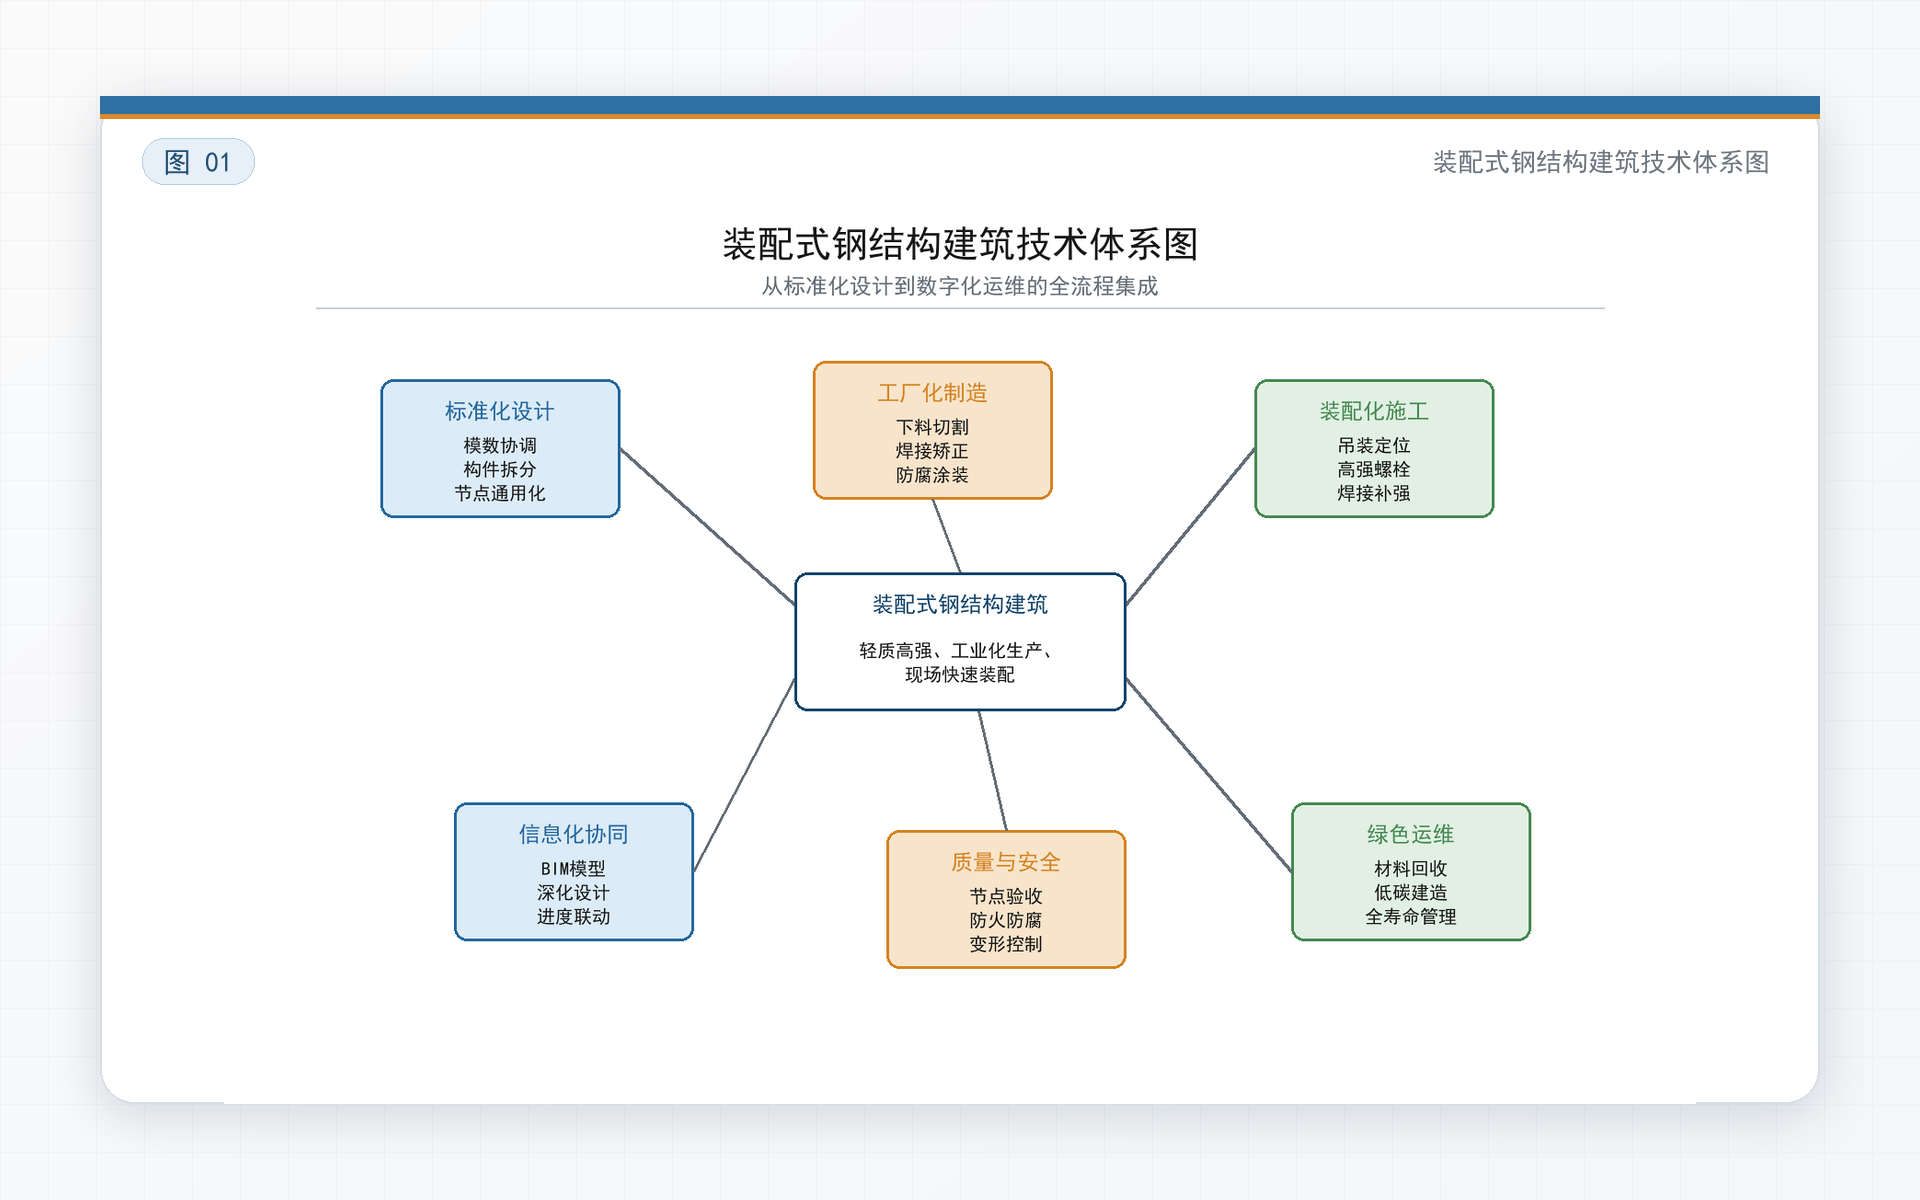
\includegraphics[width=0.94\linewidth]{figures_beautified/fig01_technology_system_beautified.png}
  \caption{装配式钢结构建筑技术体系图}
  \label{fig:fig01-technology-system-beautified}
\end{figure}

% 钢构件工厂制造流程图
\begin{figure}[htbp]
  \centering
  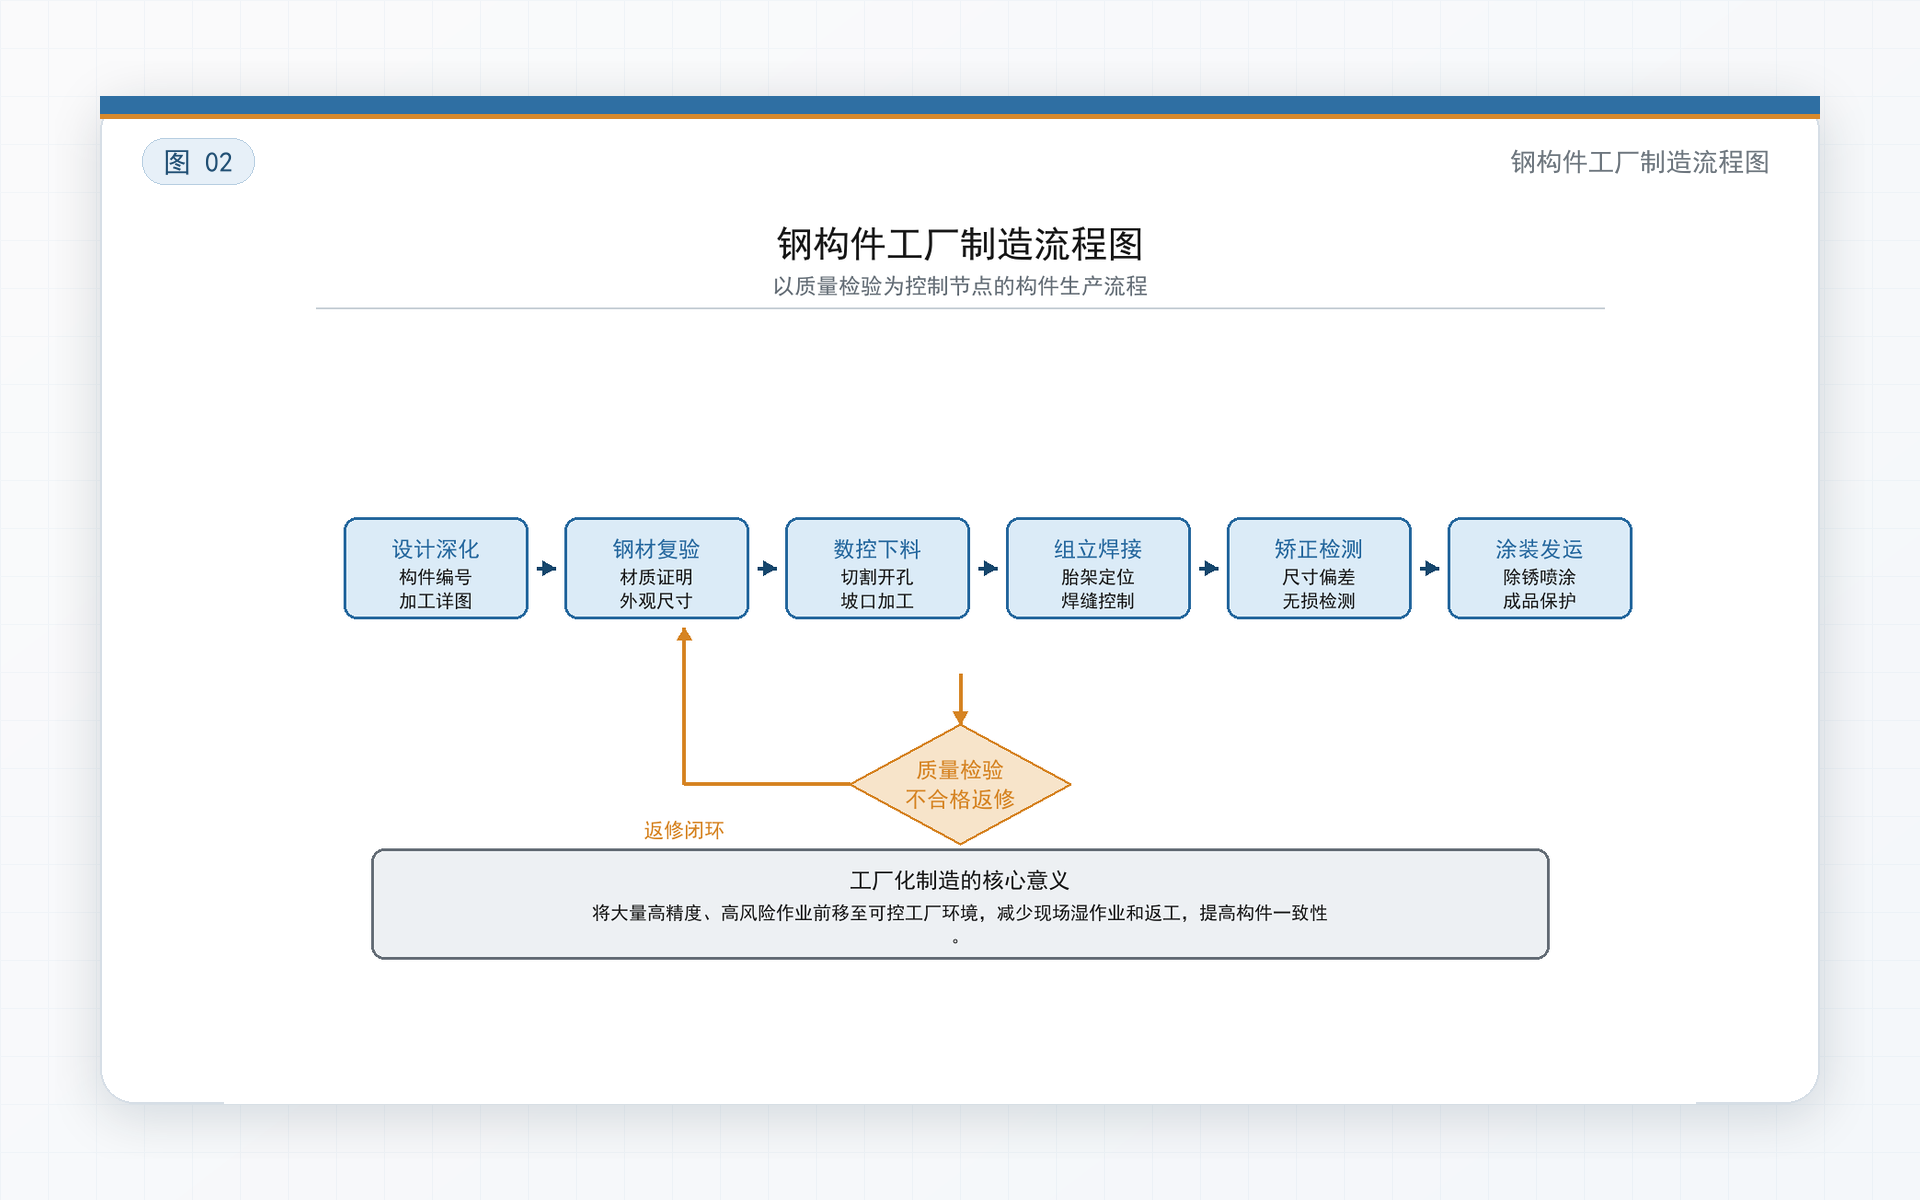
\includegraphics[width=0.94\linewidth]{figures_beautified/fig02_factory_manufacturing_beautified.png}
  \caption{钢构件工厂制造流程图}
  \label{fig:fig02-factory-manufacturing-beautified}
\end{figure}

% 现场吊装与装配施工流程图
\begin{figure}[htbp]
  \centering
  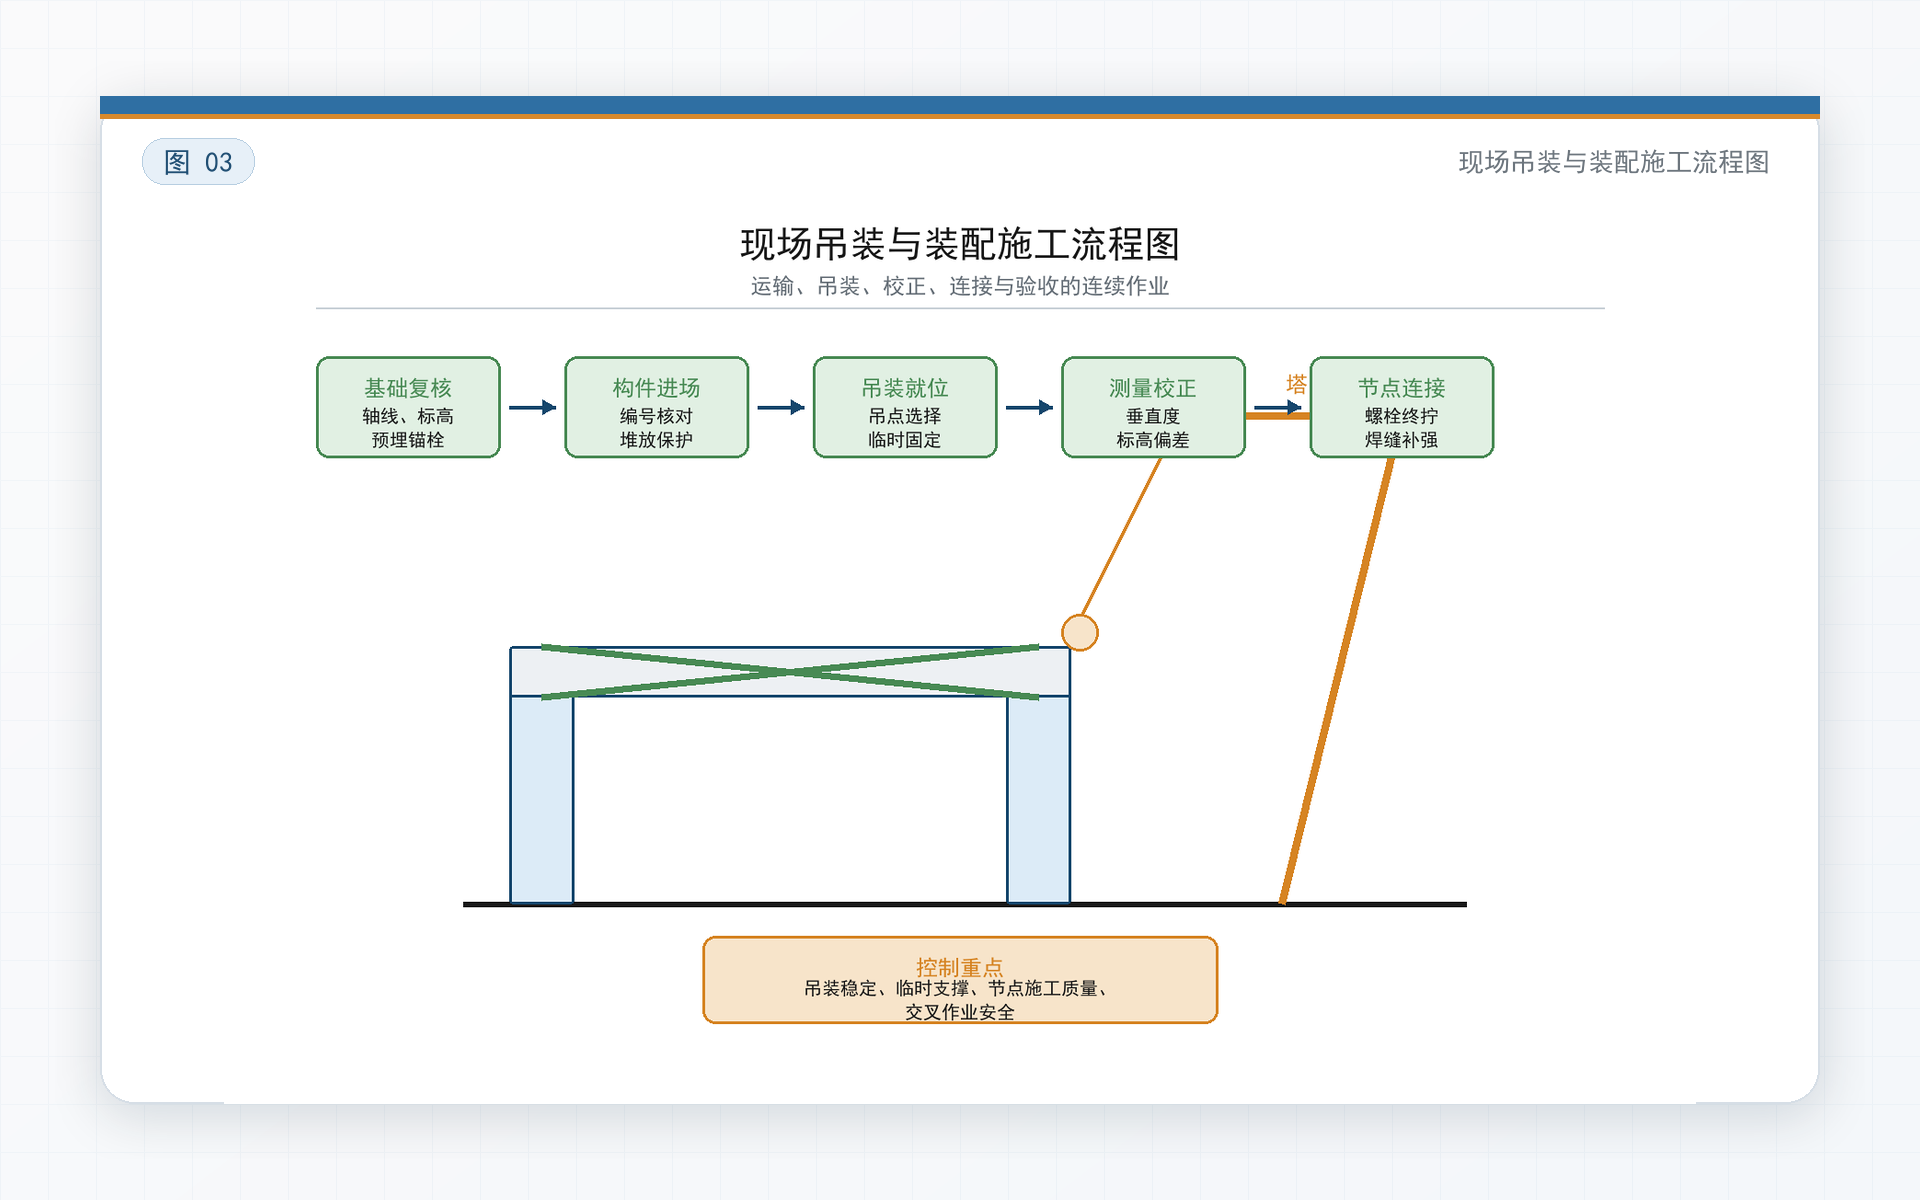
\includegraphics[width=0.94\linewidth]{figures_beautified/fig03_site_assembly_beautified.png}
  \caption{现场吊装与装配施工流程图}
  \label{fig:fig03-site-assembly-beautified}
\end{figure}

% 梁柱螺栓连接节点示意图
\begin{figure}[htbp]
  \centering
  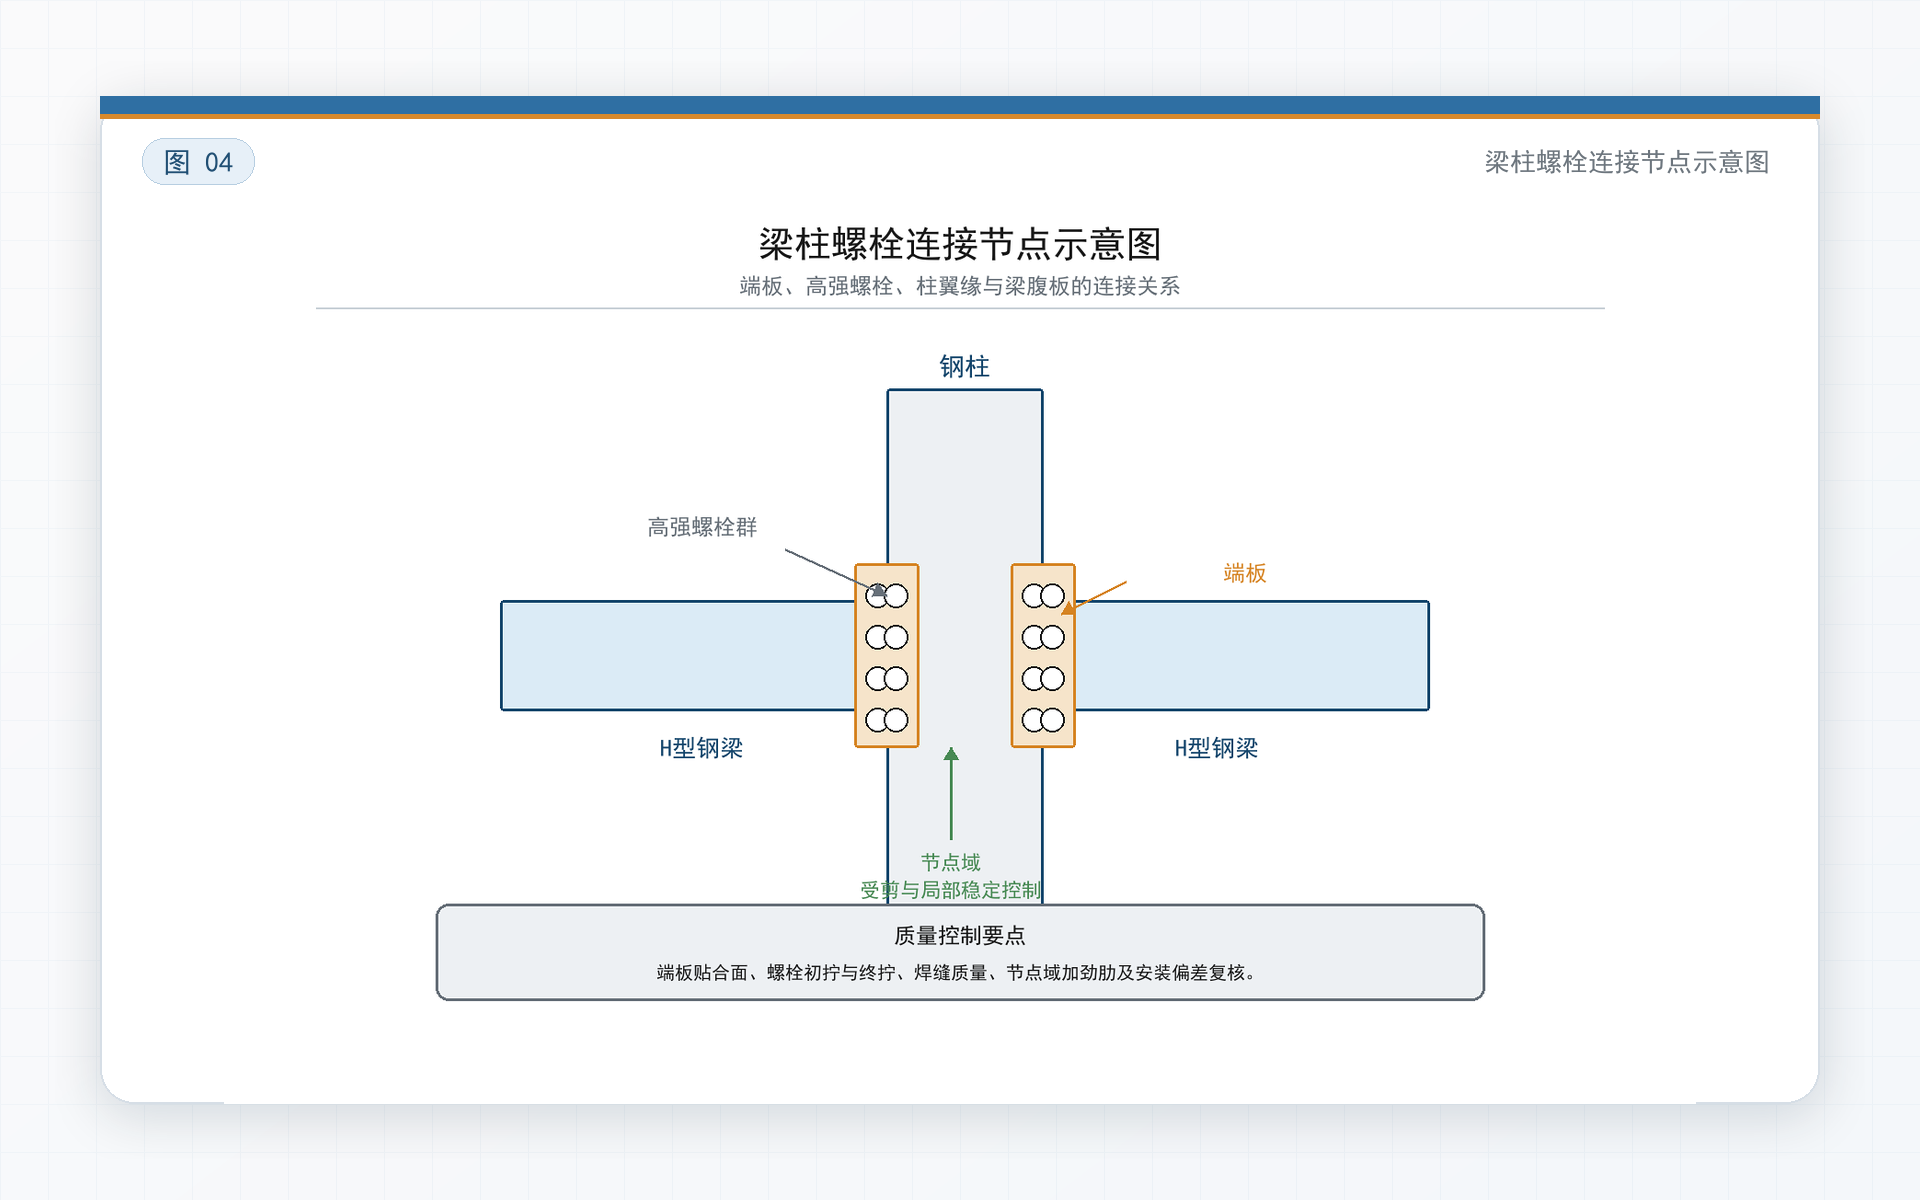
\includegraphics[width=0.94\linewidth]{figures_beautified/fig04_beam_column_joint_beautified.png}
  \caption{梁柱螺栓连接节点示意图}
  \label{fig:fig04-beam-column-joint-beautified}
\end{figure}

% 钢框架-支撑结构受力路径示意图
\begin{figure}[htbp]
  \centering
  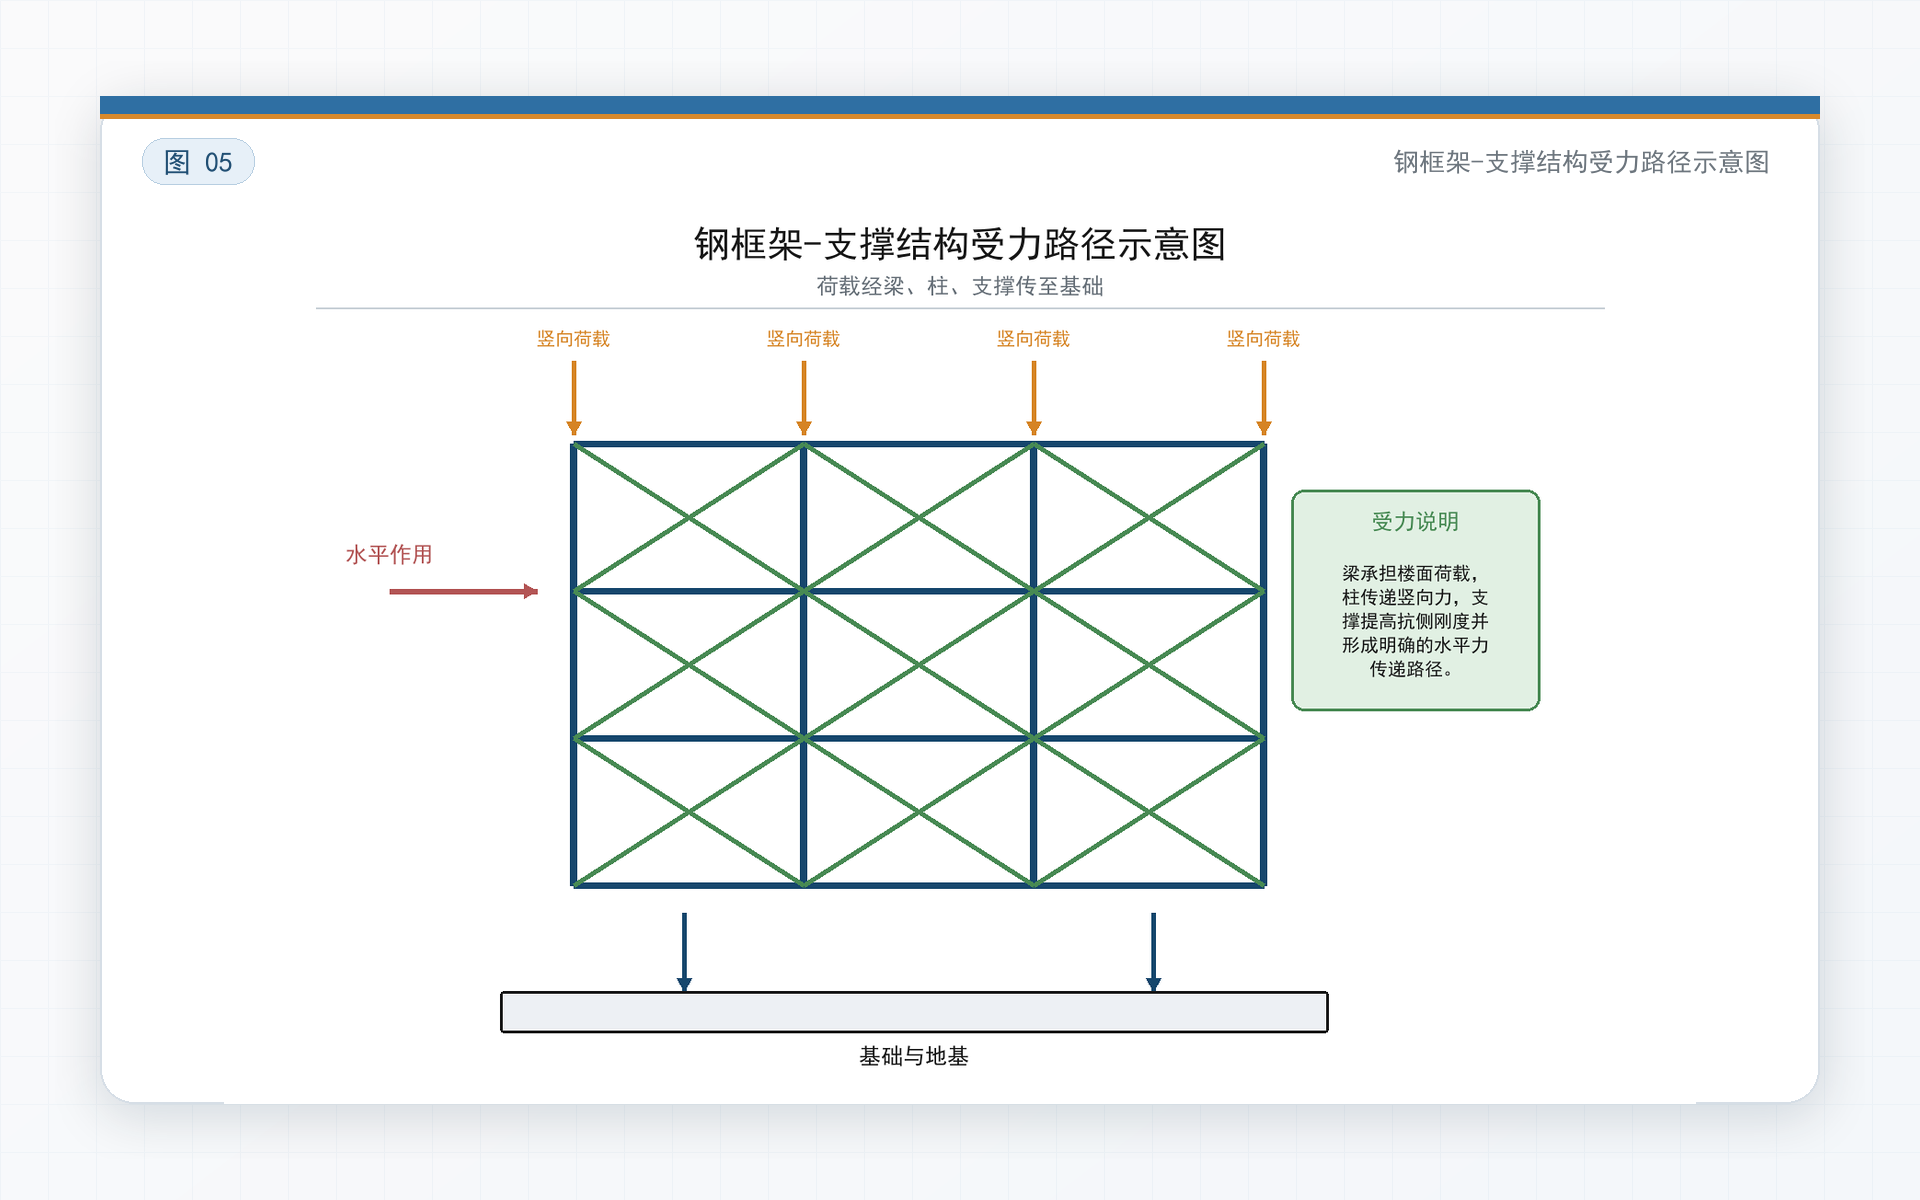
\includegraphics[width=0.94\linewidth]{figures_beautified/fig05_force_path_beautified.png}
  \caption{钢框架-支撑结构受力路径示意图}
  \label{fig:fig05-force-path-beautified}
\end{figure}

% 楼承板组合楼盖构造示意图
\begin{figure}[htbp]
  \centering
  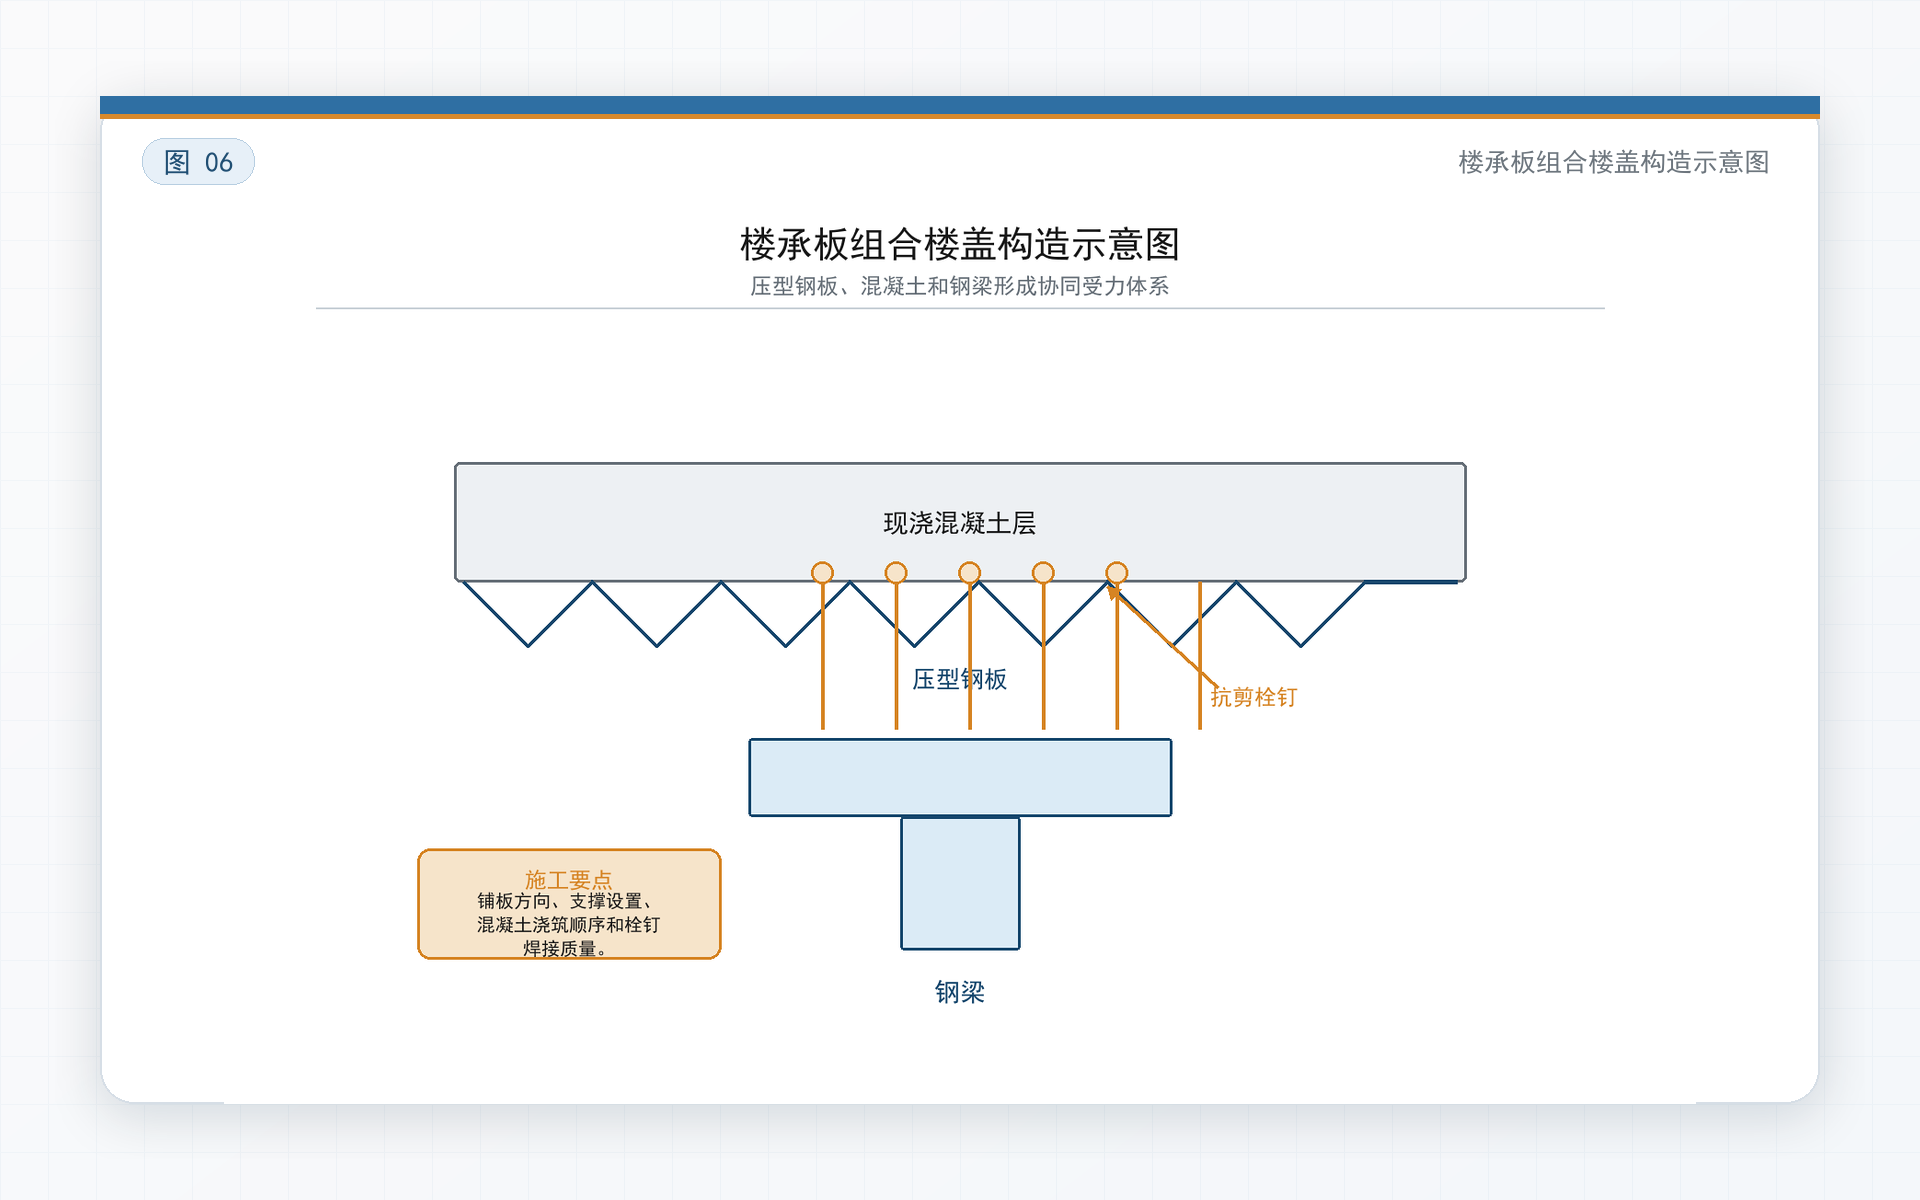
\includegraphics[width=0.94\linewidth]{figures_beautified/fig06_composite_floor_beautified.png}
  \caption{楼承板组合楼盖构造示意图}
  \label{fig:fig06-composite-floor-beautified}
\end{figure}

% 钢结构防火保护构造示意图
\begin{figure}[htbp]
  \centering
  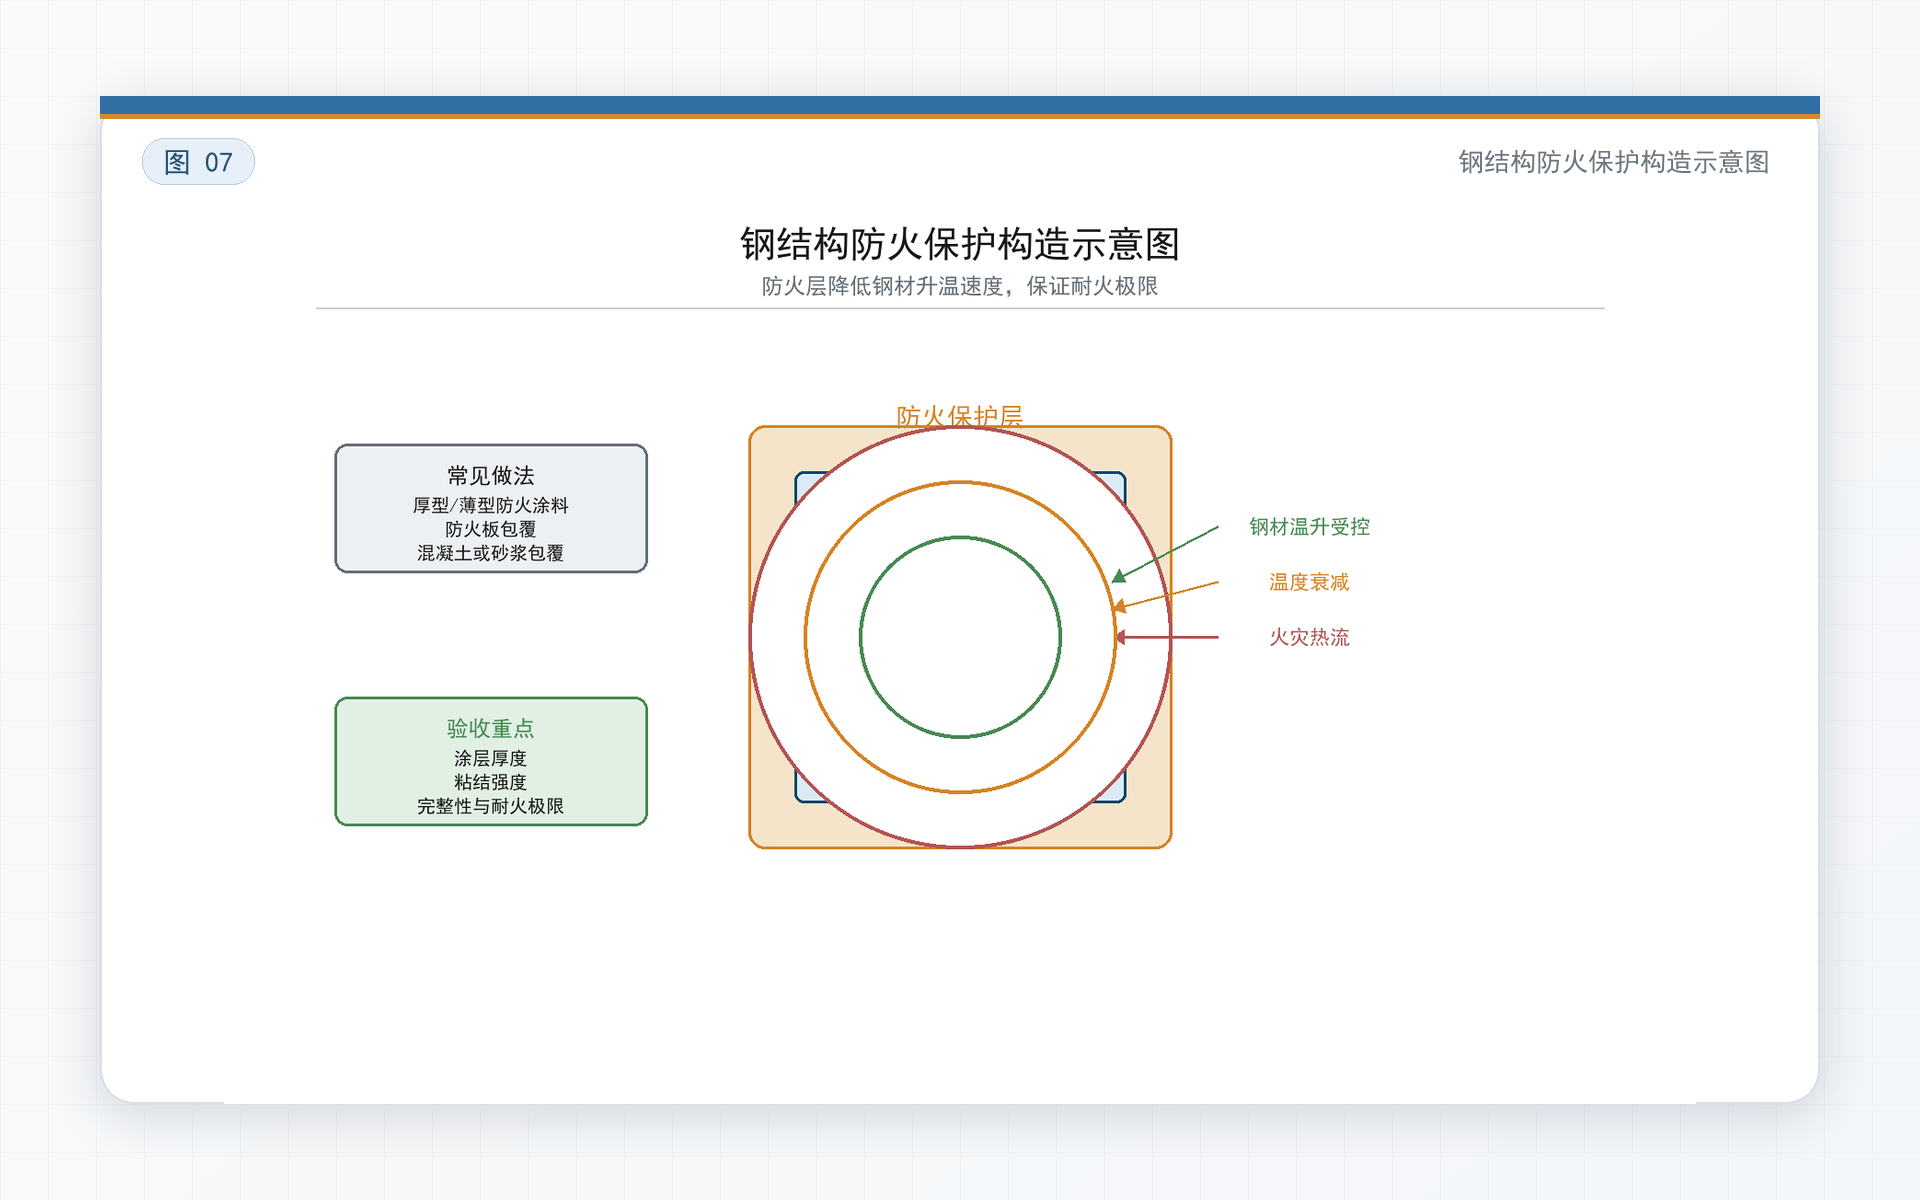
\includegraphics[width=0.94\linewidth]{figures_beautified/fig07_fire_protection_beautified.png}
  \caption{钢结构防火保护构造示意图}
  \label{fig:fig07-fire-protection-beautified}
\end{figure}

% 钢结构防腐涂装层次示意图
\begin{figure}[htbp]
  \centering
  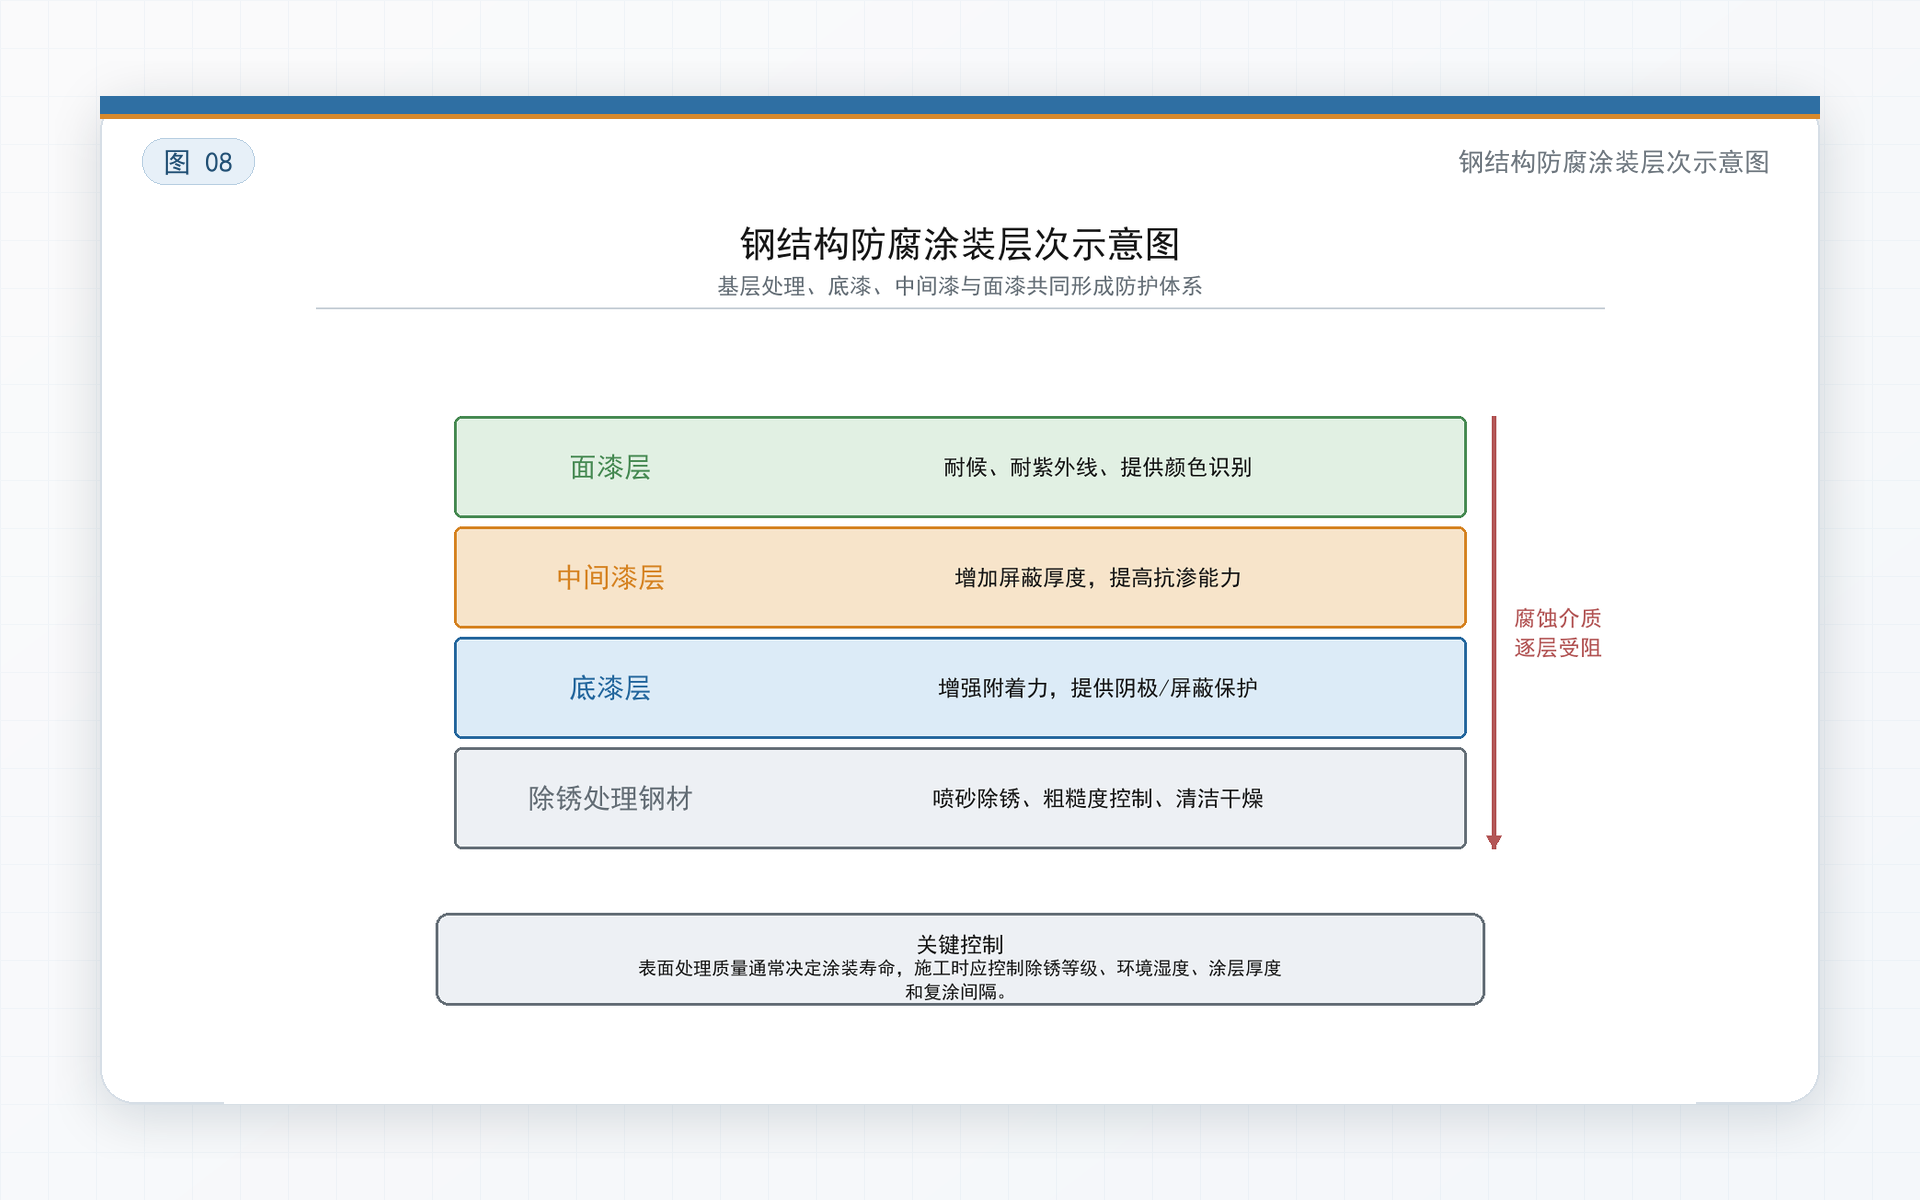
\includegraphics[width=0.94\linewidth]{figures_beautified/fig08_anticorrosion_layers_beautified.png}
  \caption{钢结构防腐涂装层次示意图}
  \label{fig:fig08-anticorrosion-layers-beautified}
\end{figure}

% BIM协同设计、制造、施工流程图
\begin{figure}[htbp]
  \centering
  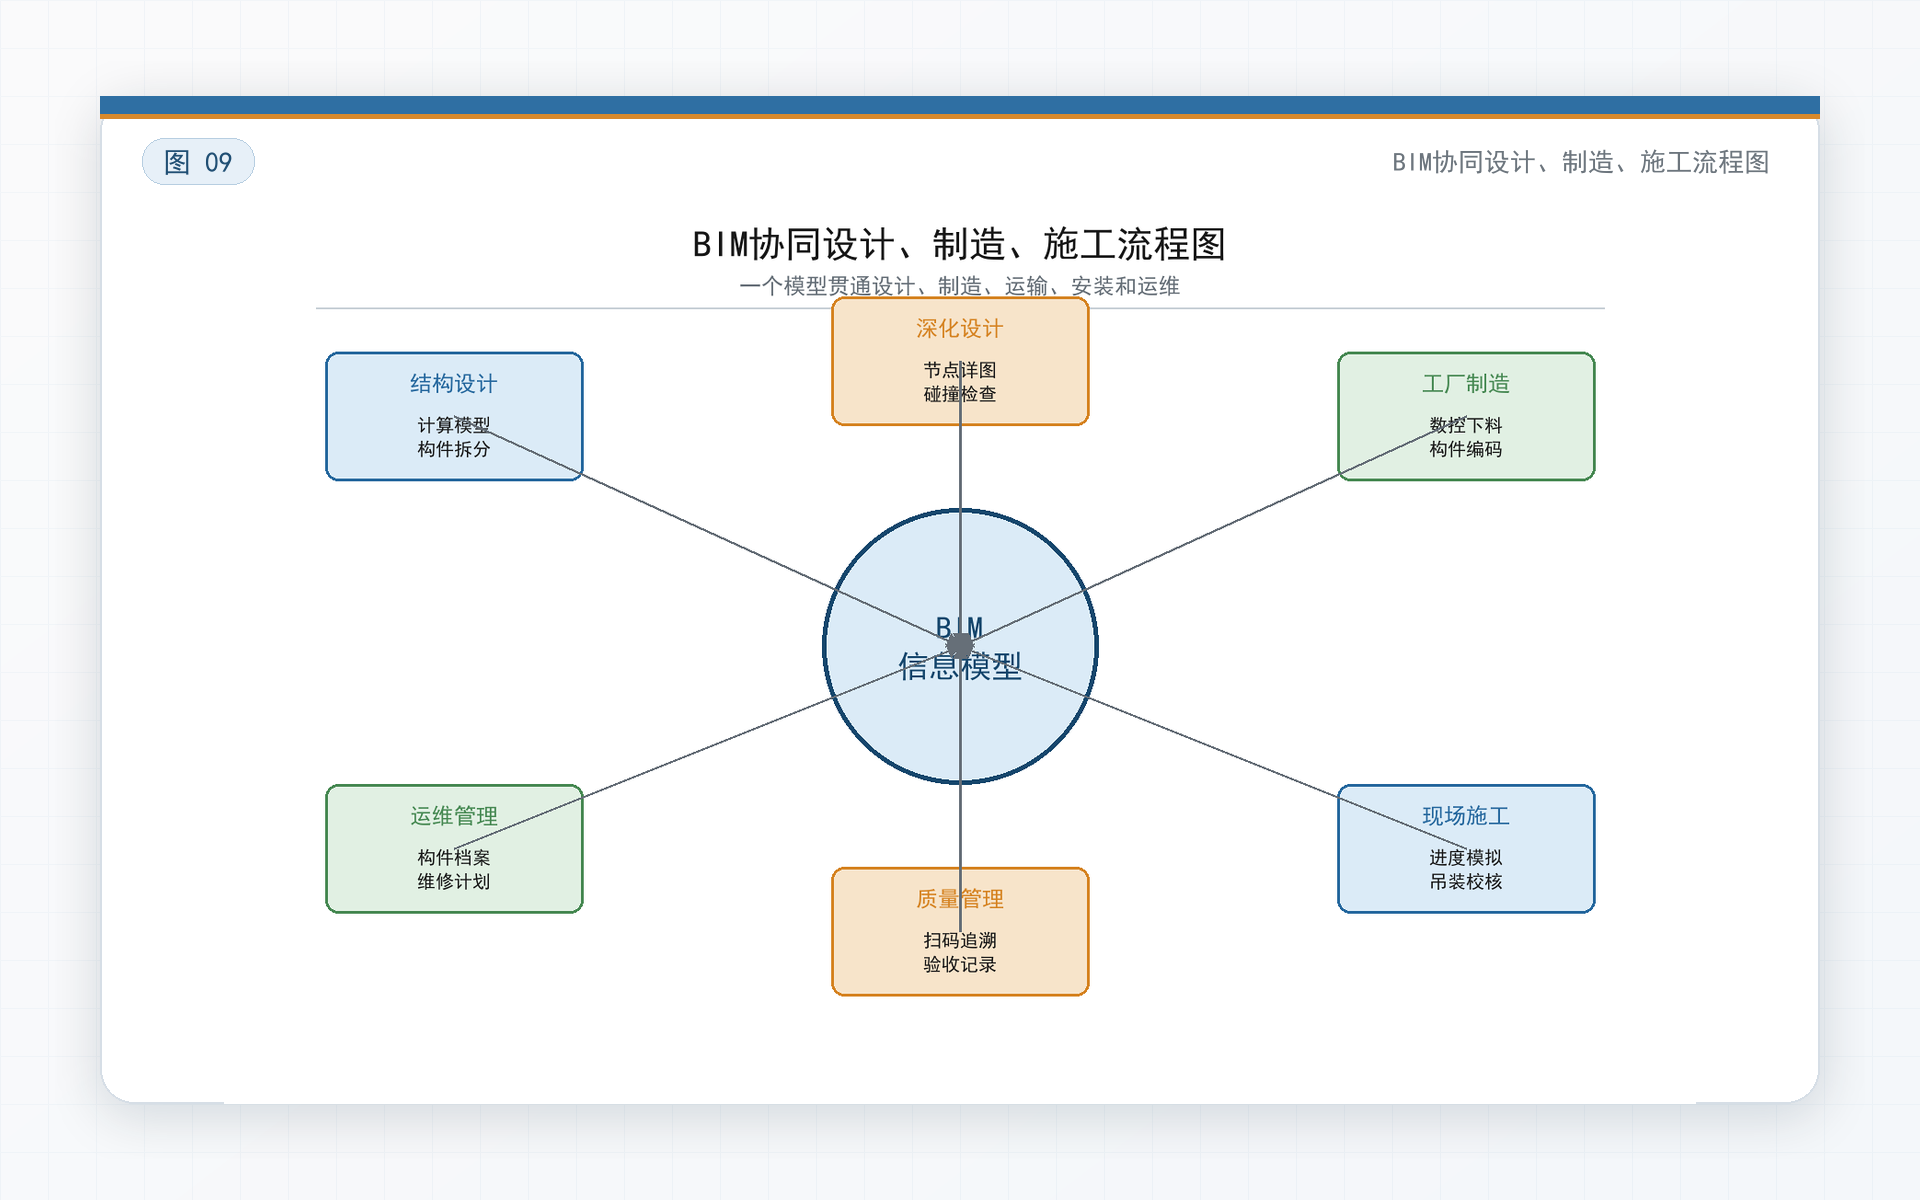
\includegraphics[width=0.94\linewidth]{figures_beautified/fig09_bim_collaboration_beautified.png}
  \caption{BIM协同设计、制造、施工流程图}
  \label{fig:fig09-bim-collaboration-beautified}
\end{figure}

% 装配式钢结构质量控制闭环图
\begin{figure}[htbp]
  \centering
  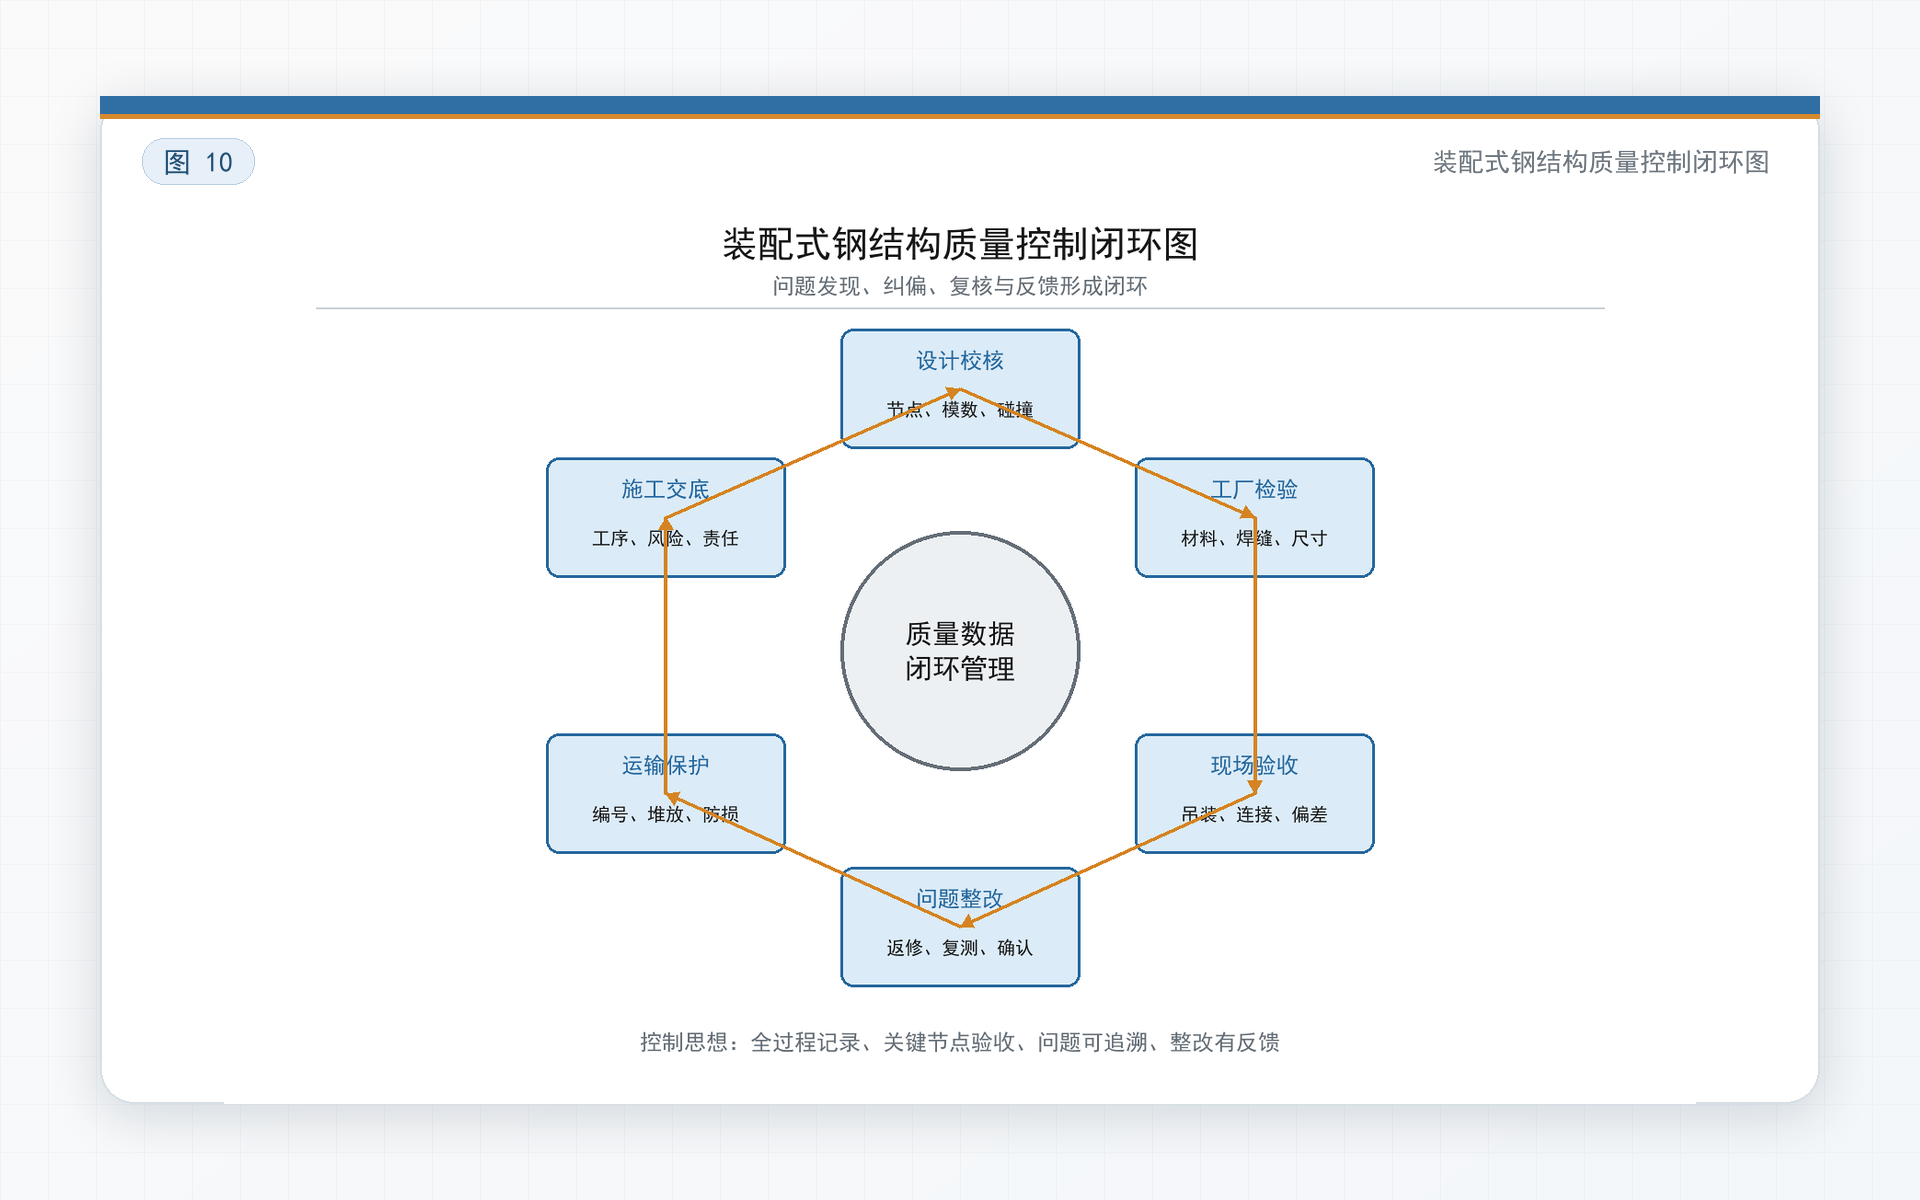
\includegraphics[width=0.94\linewidth]{figures_beautified/fig10_quality_control_loop_beautified.png}
  \caption{装配式钢结构质量控制闭环图}
  \label{fig:fig10-quality-control-loop-beautified}
\end{figure}

% 装配式钢结构绿色建造优势示意图
\begin{figure}[htbp]
  \centering
  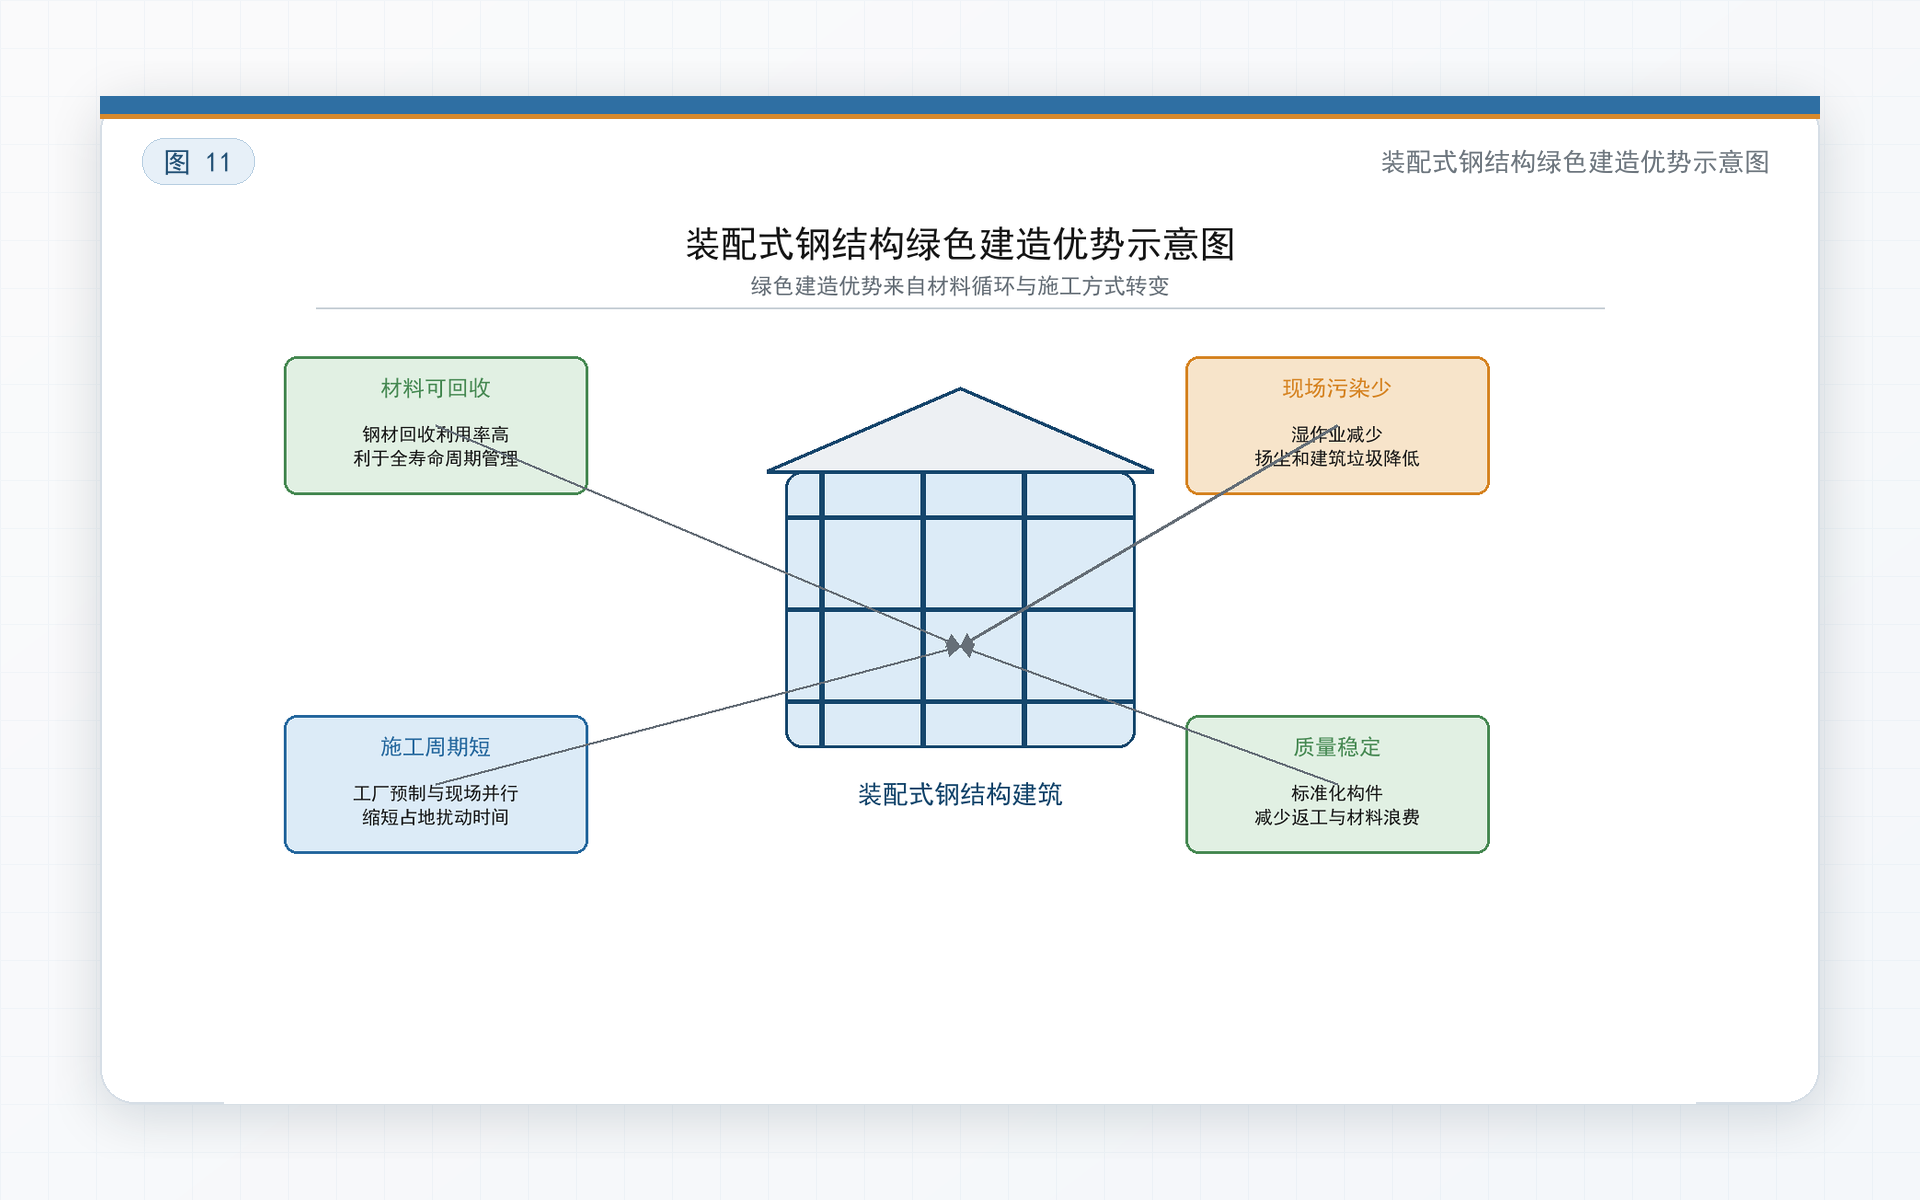
\includegraphics[width=0.94\linewidth]{figures_beautified/fig11_green_construction_beautified.png}
  \caption{装配式钢结构绿色建造优势示意图}
  \label{fig:fig11-green-construction-beautified}
\end{figure}

% 装配式钢结构未来发展趋势路线图
\begin{figure}[htbp]
  \centering
  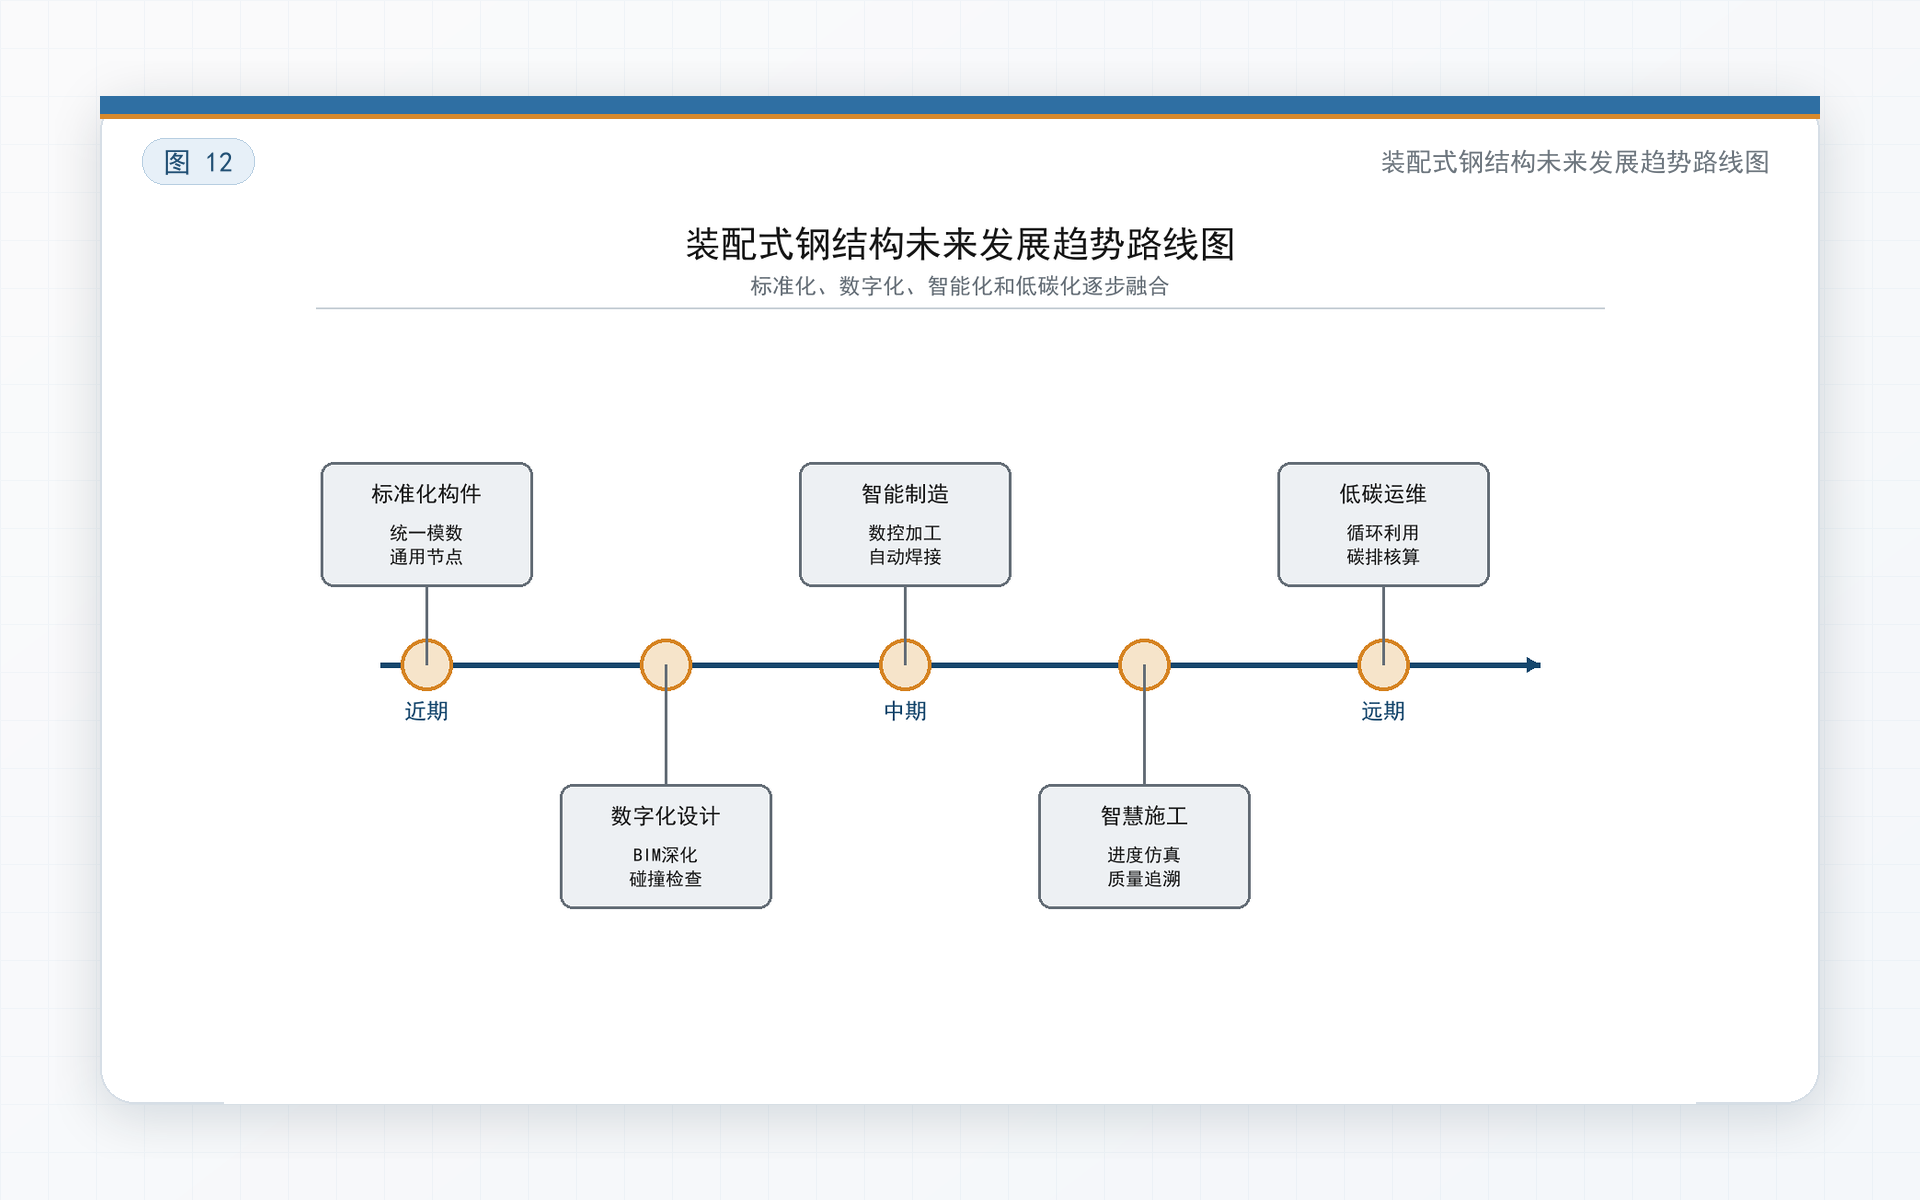
\includegraphics[width=0.94\linewidth]{figures_beautified/fig12_development_roadmap_beautified.png}
  \caption{装配式钢结构未来发展趋势路线图}
  \label{fig:fig12-development-roadmap-beautified}
\end{figure}

% 传统现浇建筑与装配式钢结构施工流程对比图
\begin{figure}[htbp]
  \centering
  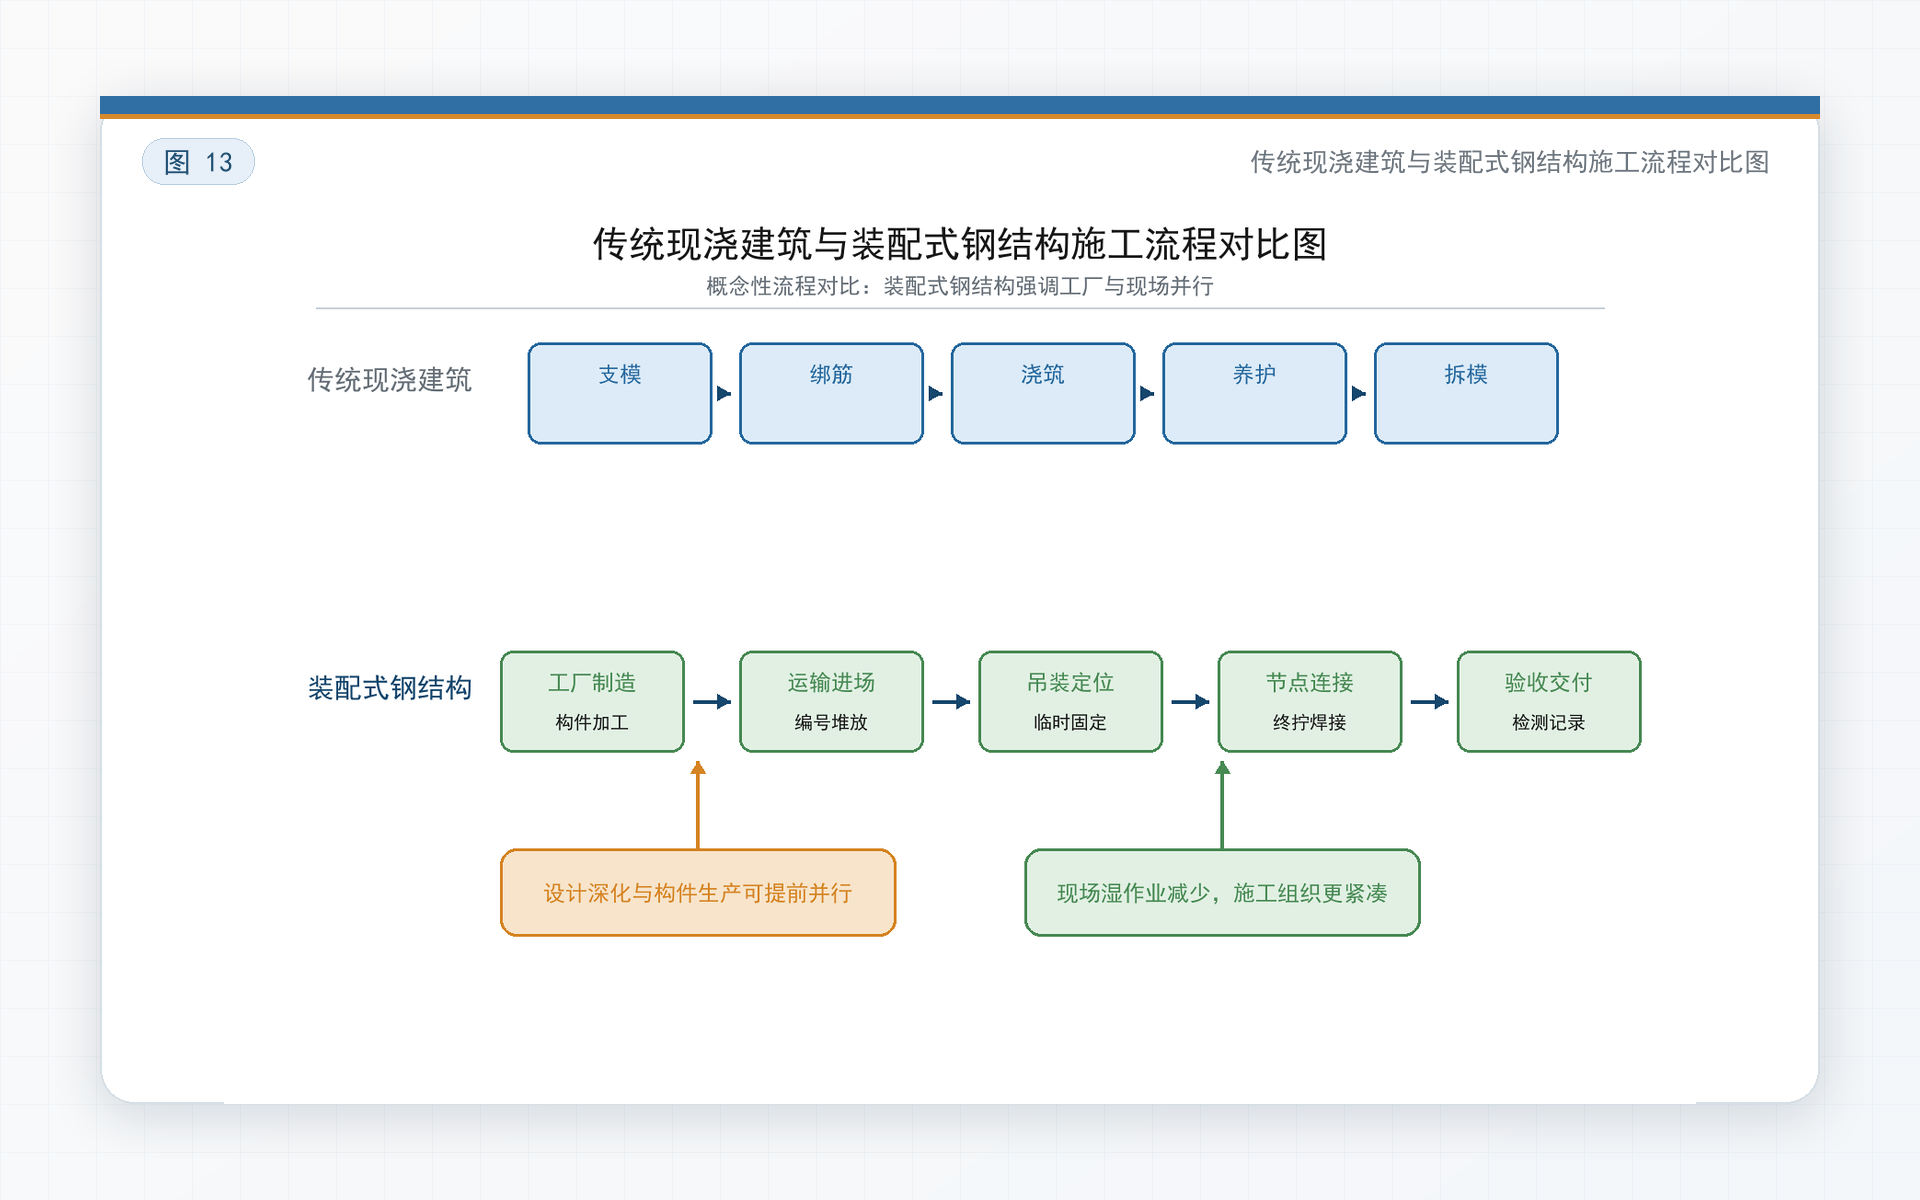
\includegraphics[width=0.94\linewidth]{figures_beautified/fig13_process_comparison_beautified.png}
  \caption{传统现浇建筑与装配式钢结构施工流程对比图}
  \label{fig:fig13-process-comparison-beautified}
\end{figure}

% 钢结构、混凝土结构、木结构综合特点对比雷达图
\begin{figure}[htbp]
  \centering
  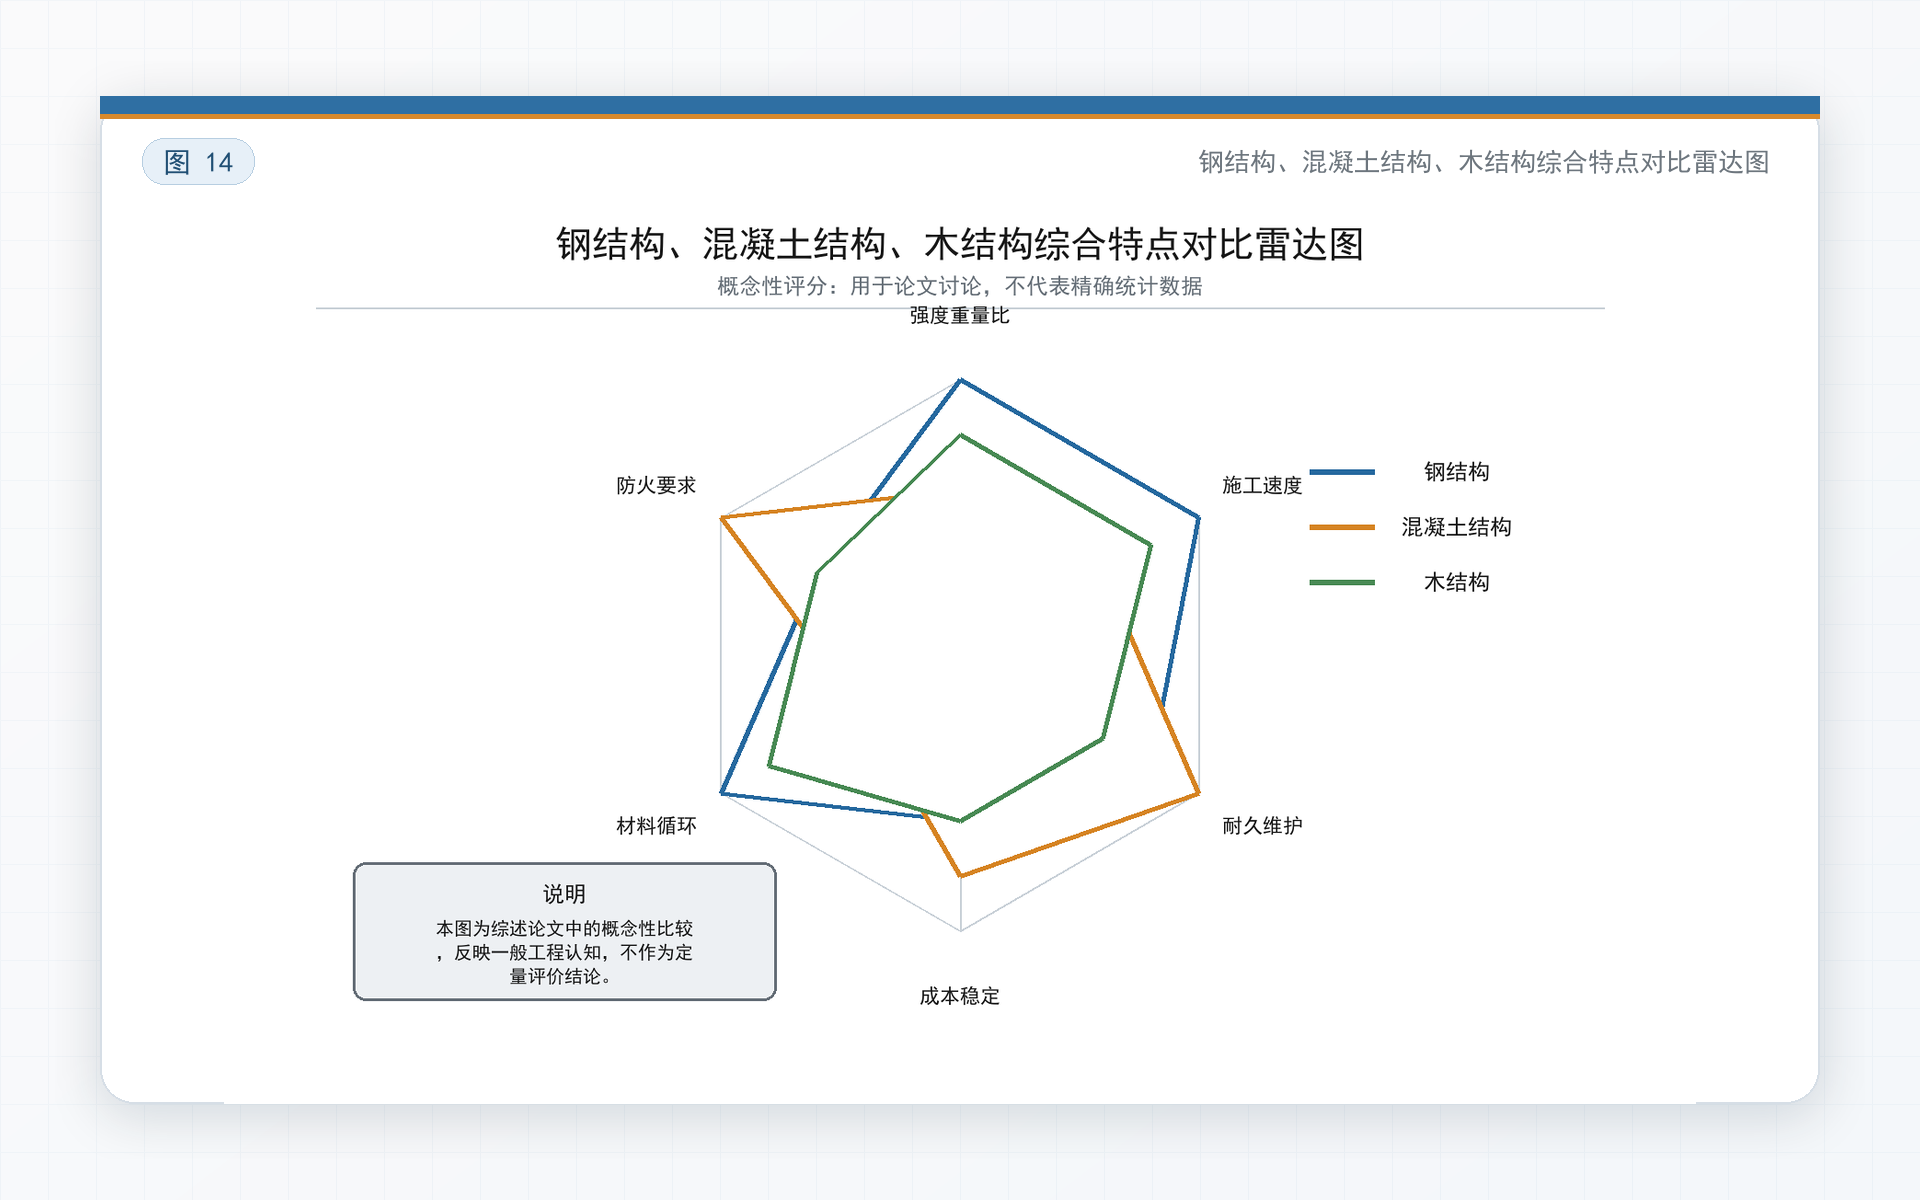
\includegraphics[width=0.94\linewidth]{figures_beautified/fig14_structure_radar_beautified.png}
  \caption{钢结构、混凝土结构、木结构综合特点对比雷达图}
  \label{fig:fig14-structure-radar-beautified}
\end{figure}

% 装配式钢结构推广影响因素权重示意图
\begin{figure}[htbp]
  \centering
  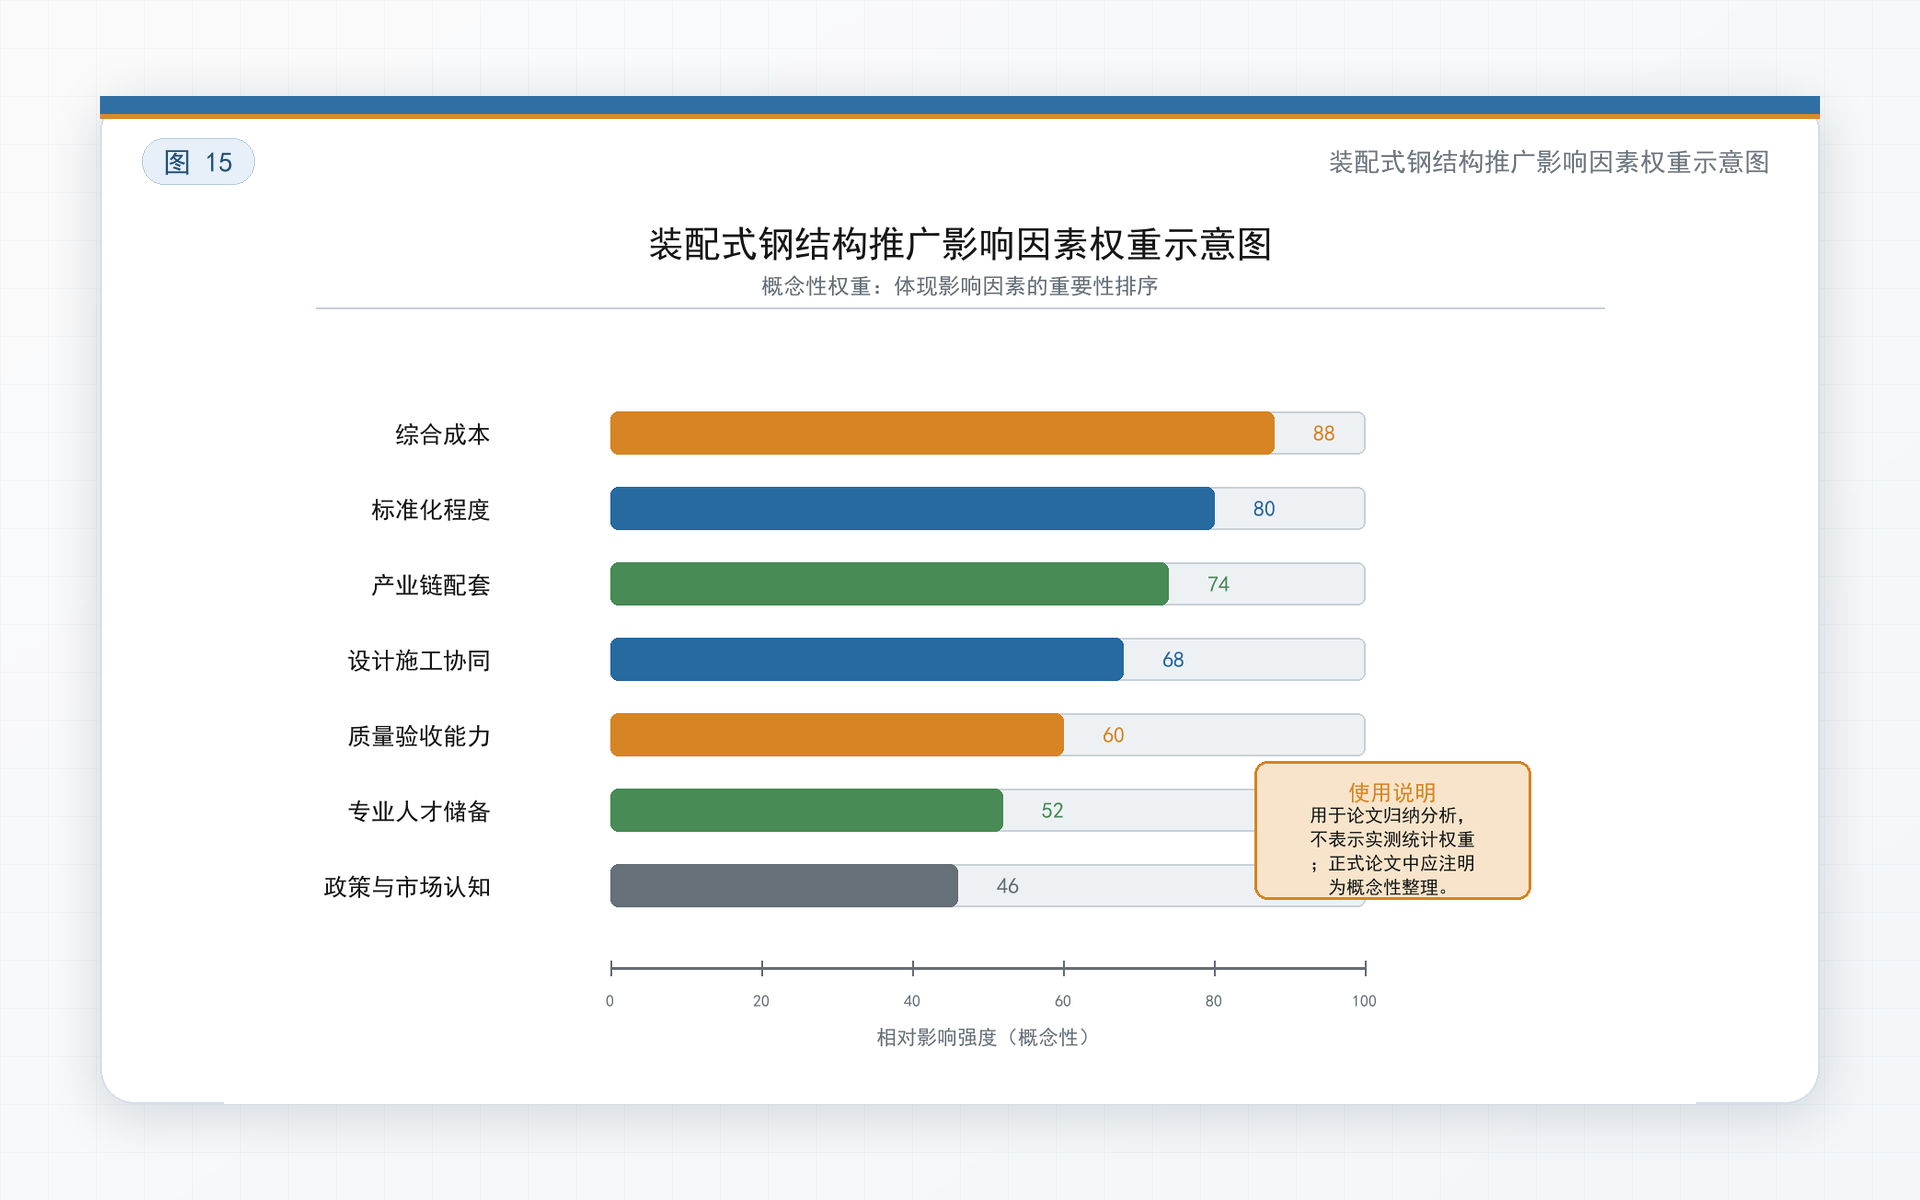
\includegraphics[width=0.94\linewidth]{figures_beautified/fig15_adoption_factors_beautified.png}
  \caption{装配式钢结构推广影响因素权重示意图}
  \label{fig:fig15-adoption-factors-beautified}
\end{figure}
